\chapter{2D Systems}\label{ch:2Dsyst}
The previous chapters considered systems distributed over one spatial dimension. As not all musical instruments or instrument-components can be simplified to this, higher dimensional systems need to be taken into consideration, such as 2D systems. 2D PDEs can be used to model drum membranes, plate reverbs or simplified instrument bodies. 

Apart from being slightly more complex than 1D models, the main issue with 2D systems is that their implementations are orders of magnitude heavier to compute than 1D schemes. This chapter will therefore also provide details on how to best implement these schemes in \texttt{MATLAB}. Implementation in C++ will be detailed in Chapter \ref{ch:realtime}.

This chapter starts by providing some additional information about 2D grid functions and operators. Then, the 2D wave equation is presented, which is used to extend the analysis techniques presented in Chapter \ref{ch:analysis} to 2D.\footnote{The abbreviation 2D will also be used for `two dimensions'.} Afterwards, two 2D models used in this work: the thin plate and the stiff membrane, will be described in a similar fashion.
The systems modelled in this work are simplified to be rectangular and are defined on a Cartesian coordinate system. Section \ref{sec:radialCoordinates} briefly elaborates on radial coordinate systems and their shortcomings. 
Unless denoted otherwise, the theory in this chapter follows \cite{theBible}.

\section{PDEs and FD schemes in 2D}\label{sec:2Dintro}
Consider a rectangular 2D system with side lengths $L_x$ and $L_y$ (both in m) and its state described by $u = u(x,y,t)$. The system is defined for $t\geq 0$ and $(x,y) \in \D$ where domain $\D \in [0, L_x]\times [0, L_y]$ is two-dimensional. 

Similar to the 1D case explained in Section \ref{sec:gridFunctions}, the state variable can be discretised to a 2D grid function according to $u(x, y, t) \approxeq \ulmn$ with space $x = lh$ and $y = mh$ and time $t = nk$ with $k=1/\fs$. The temporal index $n\in\mathbb{N}^0$  and the spatial indices $l\in \{0, \hdots, N_x\}$ and $m\in \{0, \hdots, N_y\}$ index the grid function in space in the $x$ and $y$ directions respectively. Here, $N_x$ is the number of intervals between grid points in the $x$ direction and $N_y$ in the $y$ direction. For simplicity, the grid spacing $h$ is set to be the same in both the $x$ and $y$ directions in this work.

\subsubsection{Additional operators}
In continuous time, an additional operator referred to as the \textit{Laplacian}, can be defined as
\begin{equation}\label{eq:laplacian}
    \Delta = \pxx + \pyy,
\end{equation}
which describes a second-order spatial derivative in 2D. A 4\thOrder spatial derivative in 2D, used to model stiffness like in the stiff string in Chapter \ref{ch:stiffString}, is called the \textit{biharmonic} operator, and is defined as the Laplacian applied to itself:
\begin{equation}\label{eq:biharmonic}
    \Delta\Delta = \pxxxx + 2\pxx\pyy +  \partial_y^4.
\end{equation}

In discrete time, the same temporal and spatial shift operators as defined in Section \ref{sec:FDoperators} can be applied to grid function $\ulmn$ the latter of which only affects the spatial index $l$. Additional operators affecting spatial index $m$ for the $y$ direction are
\begin{equation}
    e_{y+}\ulmn = u_{l, m+1}^n,\quad \text{and}\quad e_{y-}\ulmn= u_{l, m-1}^n.
\end{equation}
Using these shift operators, a discrete approximation of the Laplacian in Eq. \eqref{eq:laplacian} can be made\footnote{Notice that the $\dDelta$ operator is identical to $\delta_{\Delta \boxplus}$ in \cite{theBible}, but will not be used here as Eq. \eqref{eq:discreteLaplacian} is the only discretisation to the $\Delta$ operator used in this work.} 
\begin{equation}\label{eq:discreteLaplacian}
    \Delta \approxeq \dDelta \triangleq \frac{1}{h^2}\left(e_{x+} + e_{x-} + e_{y+} + e_{y-} - 4\right),
\end{equation}
and, when applied to a grid function, yields
\begin{equation}\label{eq:laplacianExpansion}
    \Delta u \approxeq \dDelta \ulmn = \frac{1}{h^2}\left(u_{l+1, m}^n + u_{l-1, m}^n+u_{l, m+1}^n+u_{l, m-1}^n - 4 \ulmn\right). 
\end{equation}
See Figure \ref{fig:laplacian} for the stencil of the discrete Laplacian. Similarly, an approximation of the biharmonic operator in Eq. \eqref{eq:biharmonic} can be made as
\begin{equation}\label{eq:discreteBiharmonic}
% \begin{align}
        \Delta\Delta \approxeq \dDelta\dDelta 
        % &= \begin{aligned}[t]
        %     \frac{1}{h^4}\Bigg(&\left(e_{x+}^2 + 1+ e_{x+}e_{y+} + e_{x+}e_{y-} - 4e_{x+}\right)\\
        %     & + \left(1 + e_{x-}^2 + e_{x-}e_{y+} + e_{x-}e_{y-} - 4e_{x-}\right)\\
        %     & + \left(e_{x+}e_{y+} + e_{x-}e_{y+} + e_{y+}^2 + 1 - 4e_{y+}\right)\\
        %     & + \left(e_{x+}e_{y-} + e_{x-}e_{y-} + 1 + e_{y-}^2 - 4e_{y-}\right)\\
        %     & -4 \left(e_{x+} + e_{x-} + e_{y+} + e_{y-} - 4\right)\Bigg)
        % \end{aligned}\\
        \triangleq \begin{aligned}[t]
        &\frac{1}{h^4}\bigg[\left(e_{x+}^2 + e_{x-}^2 + e_{y+}^2 + e_{y-}^2\right) \\
        &\ \ \ + 2 \left(e_{x+}e_{y+} + e_{x+}e_{y-} + e_{x-}e_{y+} + e_{x-}e_{y-}\right) \\
        &\ \ \ -8 \left(e_{x+} + e_{x-} + e_{y+} + e_{y-}\right) + 20\bigg],
    \end{aligned}
% \end{align}
\end{equation}
and, when applied to a grid function, yields
\begin{equation}\nonumber
    \begin{aligned}
    \Delta\Delta u\approxeq\dDelta\dDelta \ulmn =&\frac{1}{h^4}\Big[(u_{l+2, m}^n + u_{l-2, m}^n+u_{l, m+2}^n+u_{l, m-2}^n)\\
    &\ \ \ +2(u_{l+1, m+1}^n + u_{l-1, m+1}^n+u_{l+1, m-1}^n+u_{l-1, m-1}^n)\\
    &\ \ \ -8(u_{l+1, m}^n + u_{l-1, m}^n+u_{l, m+1}^n+u_{l, m-1}^n) + 20u_{l,m}^n\Big].
    \end{aligned}
\end{equation}
See Figure \ref{fig:biharmonic} for the stencil of the discrete biharmonic operator.
\begin{figure}[h]
    \centering
    \subfloat[The $\dDelta$ operator in Eq. \eqref{eq:discreteLaplacian}.\label{fig:laplacian}]{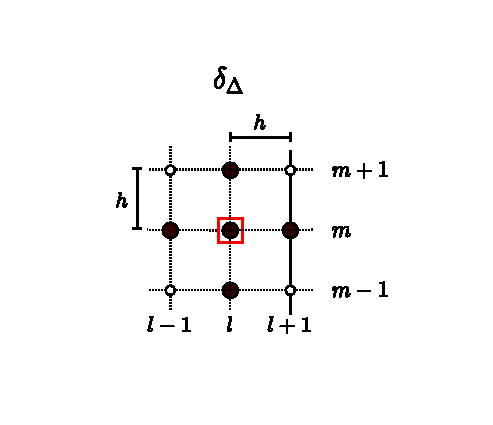
\includegraphics[width=0.45\textwidth]{figures/resonators/2d/laplacian.pdf}}\hspace{0.06\textwidth}
    \subfloat[The $\dDelta\dDelta$ operator in Eq. \eqref{eq:discreteBiharmonic}.\label{fig:biharmonic}]{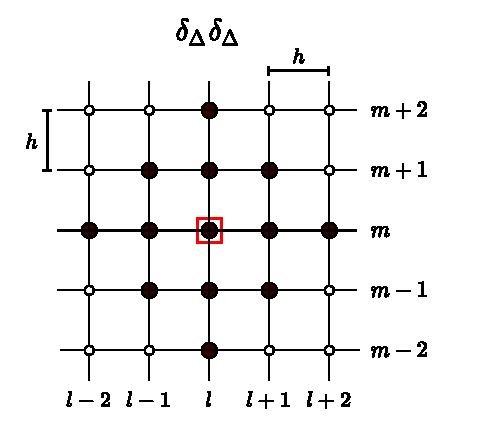
\includegraphics[width=0.45\textwidth]{figures/resonators/2d/biharmonic.pdf}}
    \caption{The stencils of the 2D spatial FD operators in Eqs. \eqref{eq:discreteLaplacian} and \eqref{eq:discreteBiharmonic} respectively. The red square denotes what grid point the operator is applied to. The stencils follow the same layout as Figure \ref{fig:operators}, but the vertical axis denotes a second spatial dimension rather than time. \label{fig:2Doperators}}
\end{figure}

\section{The 2D wave equation}\label{sec:2Dwave}
The 2D wave equation is the simplest 2D model in the context of musical acoustics and using the operators presented above it is a fairly straightforward extension to the 1D wave equation. Similar to how the 1D wave equation is used to model an ideal string, the 2D wave equation can be used to model an ideal membrane. 

The first appearance of an implementation of the 2D wave equation in a musical context was due to van Duyne and Smith who used digital waveguides, or more specifically a waveguide mesh, to discretise it \cite{Duyne1993}. The implementation is identical to the FD scheme that will be presented here.\SWcomment[though it is more general here due to $\lambda^2$ instead of hard-coded $0.5$]

This section will present the 2D wave equation in continuous time and its discretisation afterwards. The resulting FD scheme is then used as a test-case to extend the various analysis techniques presented in Chapter \ref{ch:analysis} to 2D.

\subsection{Continuous time}
Consider a system modelling the 2D wave equation with side lengths $L_x$ and $L_y$ (both in m) and its state described by $u = u(x,y,t)$. The system is defined over $(x,y) \in \D$ with domain $\D = [0, L_x] \times[0, L_y]$ and its motion is described by the following PDE:
\begin{equation}\label{eq:2DwavePDE}
    \ptt u = c^2\Delta u,
\end{equation}
with wave speed $c$ (in m/s) and the Laplacian operator as defined in Eq. \eqref{eq:laplacian}. If the 2D wave equation is used to model an ideal membrane, the wave speed is defined as $c = \sqrt{T/\rho H}$ (in m/s), with tension per unit length $T$ (in N/m), material density $\rho$ (in kg/m$^3$) and thickness $H$ (in m).

\subsubsection{Boundary conditions}
Similar to the 1D wave equation, two alternatives for boundary conditions are
\begin{subequations}\label{eq:boundaryCond2DWave}
    \begin{align}
    \begin{rightcases}
        u(0, y, t) = u(L_x, y, t) = 0\quad \forall y, \\
        u(x, 0, t) = u(x, L_y, t) = 0\quad \forall x, 
    \end{rightcases}\quad &\text{(Dirichlet, fixed)},\label{eq:contDirichlet2D}\\
    \begin{rightcases}
        \px u(0, y, t) = \px u(L_x, y, t) = 0\quad \forall y,\\
        \py u(x, 0, t) = \py u(x, L_y, t) = 0\quad \forall x, 
    \end{rightcases}\quad &\text{(Neumann, free)},\label{eq:contNeumann2D}
    \end{align}
\end{subequations}
where $\forall$ means 'for all values of'.
\subsection{Discrete time}
Using the definition for the approximation of the Laplacian in Eq. \eqref{eq:discreteLaplacian}, the 2D wave equation PDE in Eq. \eqref{eq:2DwavePDE} can be discretised to
\begin{equation}\label{eq:2DwaveFDS}
    \dtt \ulmn = c^2 \dDelta \ulmn,
\end{equation}
with $l\in\{0, \hdots, N_x\}$ and $m\in \{0, \hdots, N_y\}$ where $N_x$ and $N_y$ are the number of intervals between grid points in the $x$ and $y$ direction respectively. The operators can then be expanded (see Eq. \eqref{eq:laplacianExpansion}) and solving for $\ulm^n$ yields the following update equation 
\begin{equation}\label{eq:update2Dwave}
    \ulm^{n+1} = 2\ulmn - \ulm^{n-1} + \lambda^2 \left(u_{l+1, m}^n + u_{l-1, m}^n+u_{l, m+1}^n+u_{l, m-1}^n - 4 \ulmn\right),
\end{equation}
where the Courant number 
\begin{equation}\label{eq:courant2D}
    \lambda = \frac{ck}{h},
\end{equation}
and needs to abide
\begin{equation}\label{eq:CFL2D}
    \lambda \leq \frac{1}{\sqrt{2}}
\end{equation}
for the scheme to be stable. See Section \ref{sec:stability2Dwave} for a derivation of this. Writing this condition in terms of the grid spacing, places the following limit on $h$:
\begin{equation}\label{eq:stabilityCondition2Dwave}
    h \geq \sqrt{2}ck\,.
\end{equation}

\subsubsection{Discrete boundary conditions}
The boundary conditions in Eqs. \eqref{eq:boundaryCond2DWave} can be discretised to 
\begin{subequations}\label{eq:boundaryCond2DWaveDisc}
    \begin{align}
    \begin{rightcases}
        u_{0,m}^n = u_{N_x,m}^n = 0&&\quad \forall m, \\
        u_{l,0}^n = u_{l,N_y}^n = 0&&\quad \forall l, 
    \end{rightcases}\quad &\text{(Dirichlet, fixed)},\label{eq:discDirichlet2D}\\
    \begin{rightcases}
        \dxd u_{0,m}^n = \dxd u_{N_x,m}^n = 0&&\quad \forall m, \\
        \dyd u_{l,0}^n = \dyd u_{l,N_y}^n = 0&&\quad \forall l, 
    \end{rightcases}\quad &\text{(Neumann, free)}.\label{eq:discNeumann2D}
    \end{align}
\end{subequations}
If the Dirichlet boundary conditions are used (for all sides), the domain of calculation can simply be reduced to $l\in\{1, \hdots N_x-1\}$ and $m\in\{1, \hdots N_y-1\}$. 

\subsubsection{Stencil}
Figure \ref{fig:stencil2Dwave} shows the stencil of the 2D wave equation FD scheme in Eq. \eqref{eq:2DwaveFDS}. The grid points use the same colour-coding as previous stencils (see e.g. Figure \ref{fig:stencil1DWave}).

\begin{figure}[h]
    \centering
    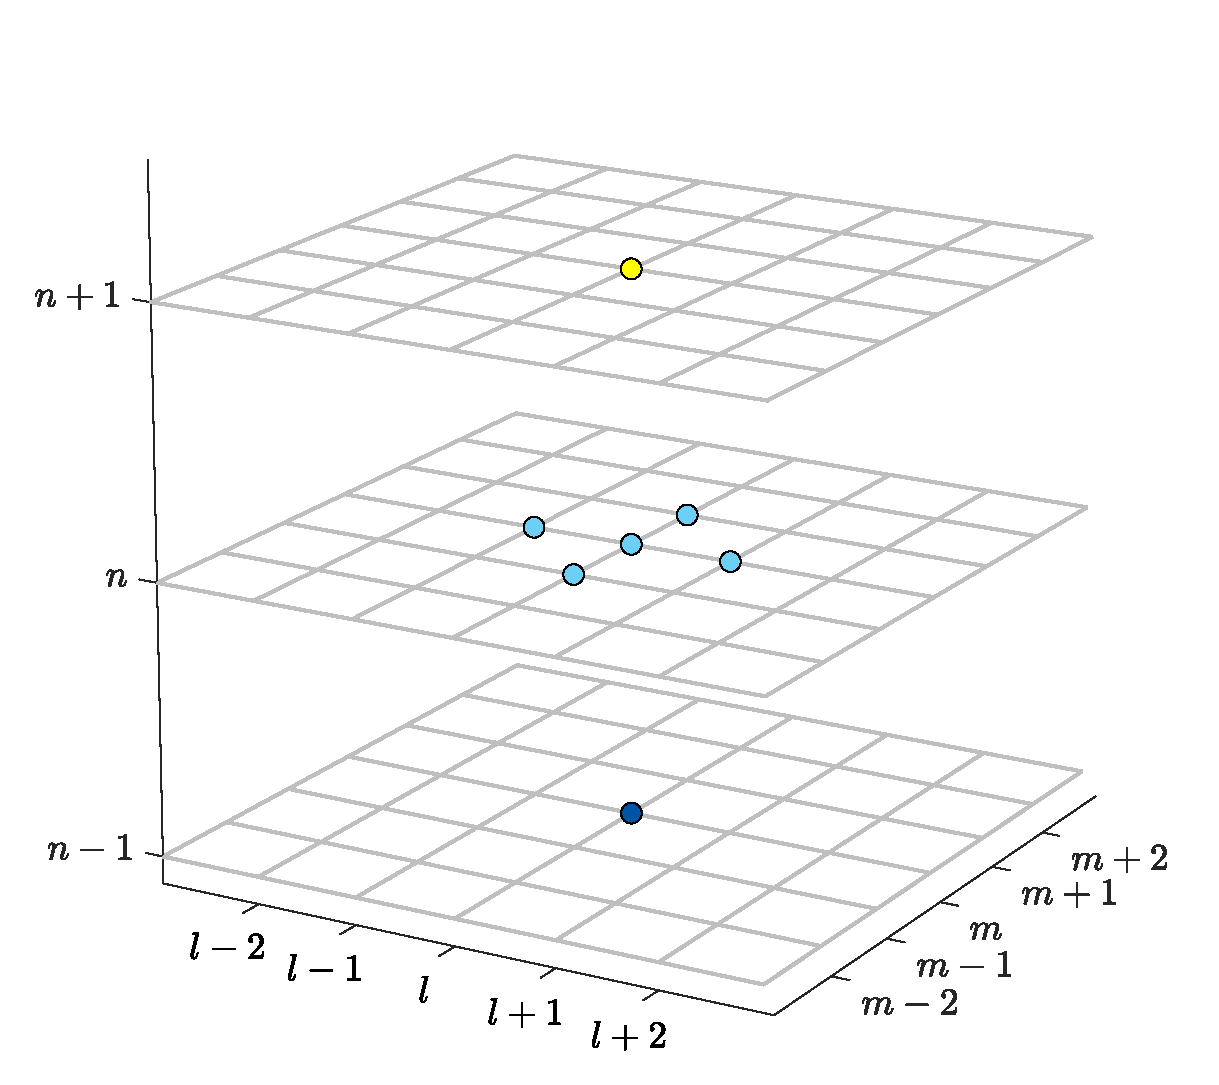
\includegraphics[width=0.7\textwidth]{figures/resonators/2d/stencil2Dwave.eps}
    \caption{The stencil for the 2D wave equation FD scheme in Eq. \eqref{eq:2DwaveFDS}. \label{fig:stencil2Dwave}}
\end{figure}
\subsection{Matrix form and output}\label{sec:2DwaveImplementation}
Similar to how the number of intervals between grid points is calculated for 1D systems in Eq. \eqref{eq:orderOfCalc}, it can be calculated in 2D using the following operations:
\begin{equation}\label{eq:orderOfCalc2D}
    h := \sqrt{2} ck, \ \ N_x := \floor[\frac{L_x}{h}], \ \  N_y := \floor[\frac{L_y}{h}], \ \  h := \text{min}\left(\frac{L_x}{N_x}, \frac{L_y}{N_y}\right), \ \  \lambda := \frac{ck}{h},
\end{equation}
where the `$\text{min}$' operator selects the smallest value of $L_x/N_x$ and $L_y/N_y$ to stay as close to the stability condition as possible. 
% Notice that the grid spacing is recalculated based the smallest value of $L_x/N_x$  $L_y/N_y$ $L/N$ for in the $x$ and $y$ direction to stay as close to the stability condition in Eq. \eqref{eq:stabilityCondition2Dwave}.
To implement the update equation in Eq. \eqref{eq:update2Dwave}, one could save the states of the system in matrices (as opposed to vectors in the 1D case such as done in Section \ref{sec:implementationStiffString}) and directly work with these. Using Dirichlet boundary conditions the $(N_x-1) \times (N_y-1)$ state matrix at time index $n$ would be
\begin{equation}
    \U^n = \begin{bmatrix}
        u^n_{1, 1} & \hdots & u^n_{1, N_x-1}\\
        \vdots & \ddots & \vdots\\
        u^n_{N_y-1, 1} & \hdots & u^n_{N_y-1, N_x-1}
    \end{bmatrix},
\end{equation}
and could be used to make a `for-loop implementation' of the update equation. This would indeed be the strategy if one would implement the scheme in e.g. C++ (see Chapter \ref{ch:realtime}). For a more compact and faster implementation in \texttt{MATLAB}, however, one could `stack' or `flatten' the state matrices to vectors and update the scheme using matrix-vector multiplication (as done for the stiff string in Section \ref{sec:implementationStiffString} for example). Again using Dirichlet boundary conditions, the stacked state vector will be structured as
\begin{equation}\label{eq:stackedState}
    \uStack^n = [(\u_{1}^n)^T, \hdots, (\u_{N_x-1}^n)^T]^T, \qwiq \u^n_l = [u^n_{l, 1}, \hdots, u^n_{l, N_y-1}]^T,
\end{equation}
and has a size of $(N_x-1)\cdot (N_y-1) \times 1$. See Figure \ref{fig:stackingMatrix} for a visualisation of the matrix-stacking process.
\begin{figure}[t]
    \centering
    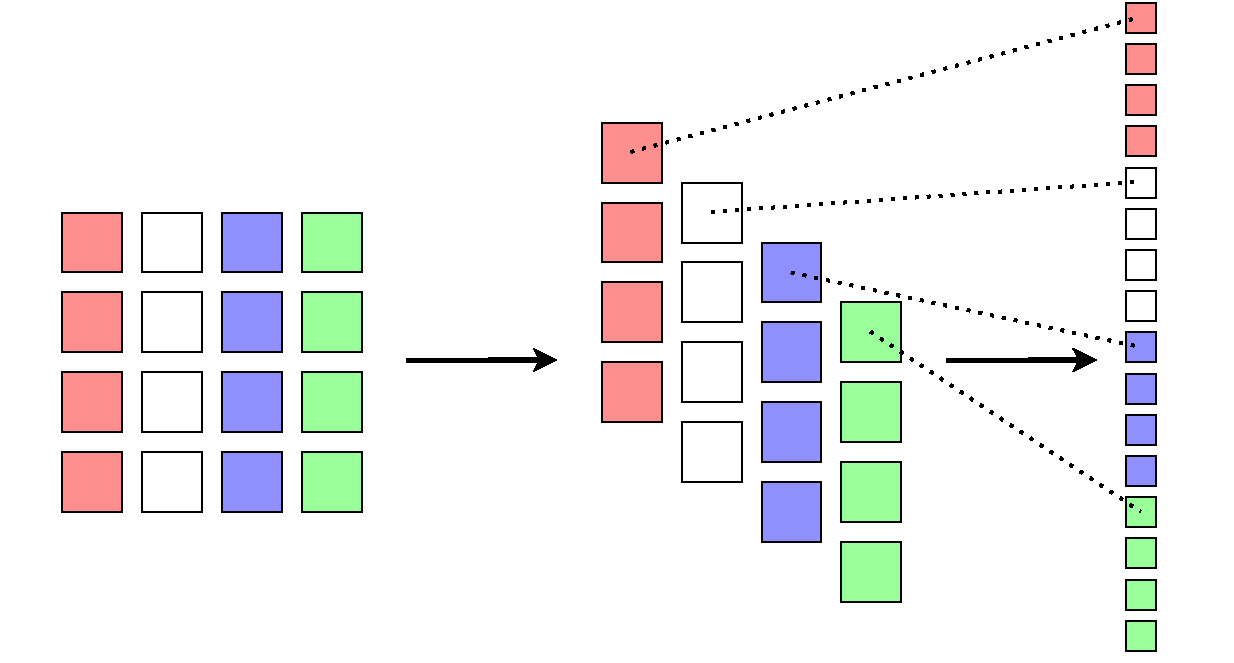
\includegraphics[width=\textwidth]{figures/resonators/2d/stackingMatrix.pdf}
    \caption{Stacking, or `flattening' a $4\times 4$ matrix to a $16$-element vector. \label{fig:stackingMatrix}}
\end{figure}

To obtain a matrix form of the $\dDelta$ operator that can be applied to this stacked state vector, the \textit{Kronecker product} and \textit{Kronecker sum} must be introduced \cite{Horn1991}. The Kronecker product between two arbitrarily-sized matrices (using their dimensions as a subscript) is
\begin{equation}
    \A_{M\times N} \otimes \B_{K\times L} = \begin{bmatrix}
        a_{11}\B & \hdots & a_{1N}\B\\
        \vdots & \ddots & \vdots\\
        a_{M1}\B & \hdots & a_{MN}\B\\
    \end{bmatrix}_{MK \times NL}.
\end{equation}
% In essence, the Kronecker product copies a matrix $\B$ according to a matrix $\A$. gets arranged according to a 
% The matrix operators then use the Kronecker
The Kronecker sum between two square matrices is 
\begin{equation}
    \A_{M \times M} \oplus \B_{N \times N} = \I_N\otimes \A + \B \otimes\I_M,
\end{equation}
where $\I_P$ is the identity matrix of size $P\times P$. 

For Dirichlet boundary conditions, the $\Dxx$ matrix of size $(N_x-1) \times (N_x-1)$ and the $\Dyy$ matrix of size $(N_y-1) \times (N_y-1)$ can be defined (similar to Eq. \eqref{eq:DxxDef}) as
%
\setstackgap{L}{14pt}
\setstacktabbedgap{3pt}
\def\lrgap{\kern3pt}
\fixTABwidth{T}
%
\begin{equation}\label{eq:DxxyyDef}
    \Dxx = \frac{1}{h^2}\underbrace{\xbracketMatrixstack{
        -2 & 1 & & &\mathbf{0}\\
        1 & -2 & 1 & & \\
        & \ddots & \ddots & \ddots & \\
        & & 1 & -2 & 1 \\
        \mathbf{0}& & & 1 & -2 
    }}_{(N_x-1) \times (N_x-1)} \qaq \Dyy = \frac{1}{h^2}\underbrace{\xbracketMatrixstack{
        -2 & 1 & & &\mathbf{0}\\
        1 & -2 & 1 & & \\
        & \ddots & \ddots & \ddots & \\
        & & 1 & -2 & 1 \\
        \mathbf{0}& & & 1 & -2 
    }}_{(N_y-1) \times (N_y-1)}.
\end{equation}
%
Following \cite{Hamilton2016}, the matrix form of the $\dDelta$ operator can then be defined as the Kronecker sum of $\Dyy$ and $\Dxx$, yielding
%
\setstackgap{L}{14pt}
\setstacktabbedgap{2pt}
\def\lrgap{\kern3pt}
\fixTABwidth{T}
%
\begin{equation}\label{eq:DDeltaMatrix}
    \DDeltamat = \Dyy \oplus \Dxx = \xbracketMatrixstack{
        \ddots & & & & \mathbf{0}\\
        &\Dyy & & & \\
        & &\Dyy & & \\
        & & & \Dyy & \\
        \mathbf{0}& & & & \ddots
    } + \frac{1}{h^2}\!\!\xbracketMatrixstack{
         \ddots&\ddots & & & \mathbf{0}\\
         \ddots&-2\I&\I & & \\
        &\I&-2\I &\I &  \\
        & & \I& -2\I &\ddots\\
        \mathbf{0}& & & \ddots& \ddots
    },
\end{equation}
where the identity matrix $\I = \I_{N_x-1}$. The $\DDeltamat$ matrix is square and of size $(N_x-1)\cdot (N_y-1)\times (N_x-1)\cdot (N_y-1)$.

Using the above, the FD scheme in Eq. \eqref{eq:2DwaveFDS} can then be compactly written in matrix form as
\begin{equation}\label{eq:matrixUpdate2Dwave}
    \uStack^{n+1} = \left(2 \I + c^2k^2 \DDeltamat\right) \uStack^n - \uStack^{n-1},
\end{equation}
where the identity matrix is of the same size as $\DDeltamat$. See Appendix \ref{app:2DWave} for a \texttt{MATLAB} implementation of the 2D wave equation.\footnote{As the matrices are extremely sparse (many $0$-entries), it is useful to utilise \texttt{MATLAB}s optimisation for sparse matrices using the \texttt{sparse()} function. One can use \texttt{speye()} for sparse identity matrices.}

If one would like to visualise the system state as a 2D grid, one can revert the stacked vector back to a matrix by using the \texttt{reshape} function in \texttt{MATLAB}:
\begin{center}
    \texttt{uMatrix = reshape(u, Ny-1, Nx-1);}
\end{center}
A 2D raised-cosine excitation can be implemented in the same way by reshaping an excitation matrix to a vector (see Section \ref{sec:2DraisedCos})\todo{check if this is still true}.

\subsubsection{Output}
Figure \ref{fig:2Dpropagation} shows the wave propagation of an implementation of the 2D wave equation with Dirichlet boundary conditions. Parameter values are $L_x = 1.5$ m, $L_y = 1$ m and $c= 360$ m/s. Waves reflect at the boundaries at an increasing rate. This is also shown in Figure \ref{fig:output2DWave}, where the output -- taken at $(x,y) = (0.15, 0.85)$ -- in time domain shows an increase in oscillations over time, due to these reflections. The right panel shows that the output contains many partials that are close together, i.e., the output is highly inharmonic. As opposed to the output of the 1D wave equation shown in Figure \ref{fig:1DWaveOutput}, where the partials are integer multiples of the fundamental frequency, the 2D wave equation exhibits aperiodic behaviour due to the aforementioned reflections, causing this inharmonicity.

\begin{figure}[h]
    \centering
    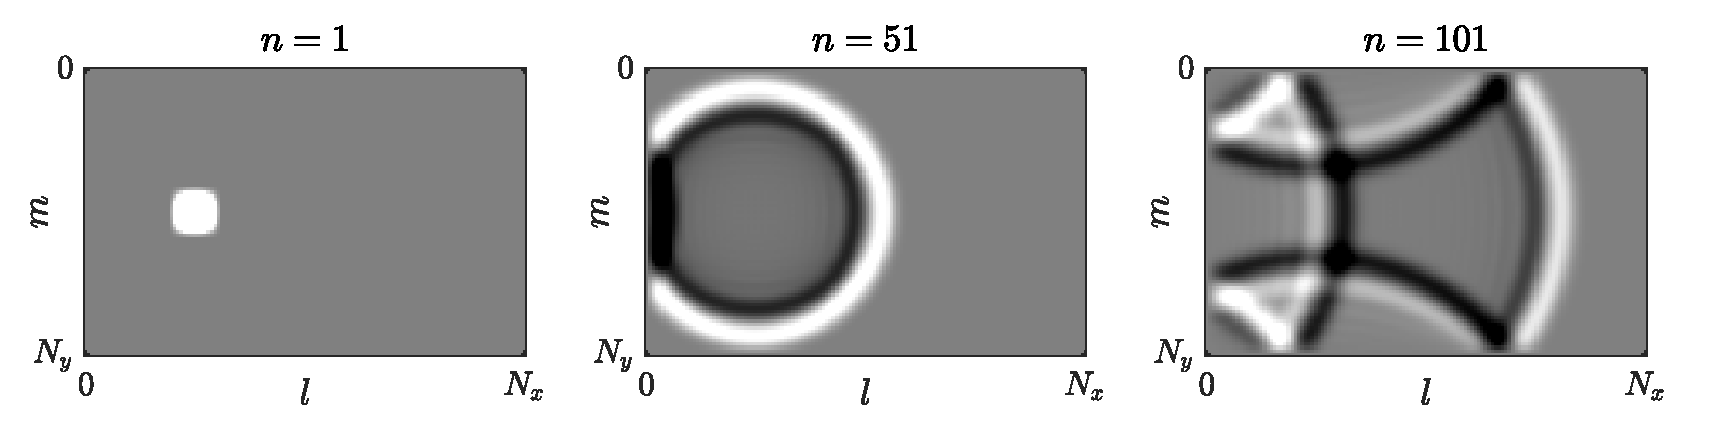
\includegraphics[width=\textwidth]{figures/resonators/2d/twoDPropagation.eps}
    \caption{Wave propagation of an implementation of the 2D wave equation with $L_x = 1.5$ m, $L_y = 1$ m and $c= 360$ m/s. The system is excited with a 2D raised cosine at $(0.25L_x, 0.5L_y)$.\label{fig:2Dpropagation}}
\end{figure}

\begin{figure}[h]
    \centering
    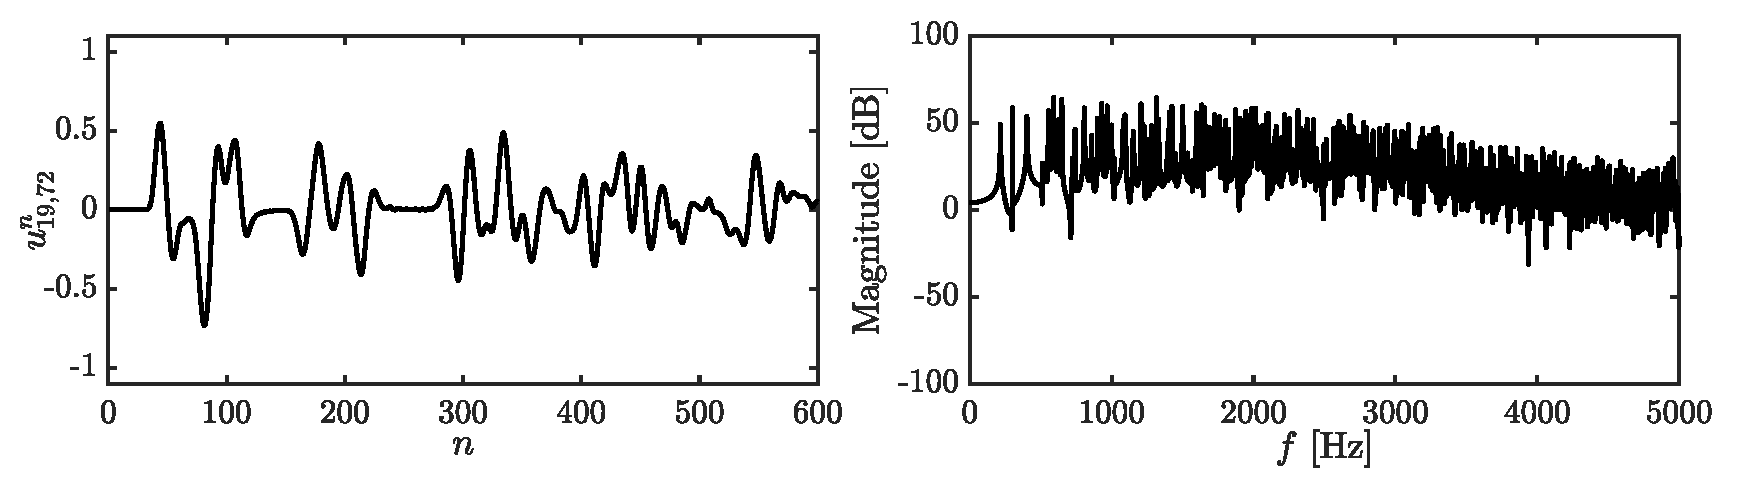
\includegraphics[width=\textwidth]{figures/resonators/2d/output2Dwave.eps}
    \caption{The output of the 2D wave equation at $(x,y) = (0.15, 0.85)$ corresponding to Figure \ref{fig:2Dpropagation}. The partials are extremely close together (notice that only frequencies up to 5000 Hz are shown) which is related to the aperiodic nature of the system behaviour. \label{fig:output2DWave}}
\end{figure}

\subsection{Frequency domain analysis in 2D}\label{sec:stability2Dwave}
Section \ref{sec:stabilityAnalysis} showed how to perform frequency domain analysis to obtain stability conditions for a FD scheme. This section shows extensions to this in 2D and follows \cite[Ch. 10]{theBible}.

In 2D, the ansatz in Eq. \eqref{eq:ansatz} can be extended to 
\begin{equation}\label{eq:2Dansatz}
    \ulmn \ansatz z^n e^{jh(l\beta_x + m\beta_y)}
\end{equation}
where $\beta_x$ and $\beta_y$ are components of a 2D wavenumber $\boldsymbol{\beta}$ in the $x$ and $y$ directions respectively. Frequency domain representations of temporal operators shown in Eq. \eqref{eq:temporalAnsatz} do not change in the 2D case. Using 
\begin{equation}\label{eq:pxpy}
    p_x = \sin^2(\beta_x h/2) \qaq p_y = \sin^2(\beta_y h/2)
\end{equation}
for brevity, the following frequency domain representation of spatial operators can be obtained through the ansatz in Eq. \eqref{eq:2Dansatz}
\begin{equation}
    \dxx \ulmn \ansatz -\frac{4}{h^2}p_x 
    \ulmn \qaq \dyy \ulmn \ansatz -\frac{4}{h^2}p_y 
    \ulmn,
\end{equation}
from which it follows that
\begin{gather}
    \dDelta\ulmn \ansatz -\frac{4}{h^2}(p_x + p_y)\ulmn,\label{eq:laplacianAnsatz}\\
    \dDelta\dDelta\ulmn \ansatz \frac{16}{h^4}(p_x + p_y)^2\ulmn.\label{eq:biharmonicAnsatz}
\end{gather}
%
Using these definitions, a frequency domain interpretation of the 2D wave equation FD scheme in Eq. \eqref{eq:2DwaveFDS} can be obtained
\begin{equation*}
    \frac{1}{k^2}\left(z - 2 +z^{-1}\right) = -\frac{4c^2}{h^2} (p_x + p_y).
\end{equation*}
Recalling $\lambda$ in Eq. \eqref{eq:courant2D}, this can be rewritten to the following characteristic equation
\begin{equation}
    z + \left(4\lambda^2(p_x + p_y)-2\right) +z^{-1} = 0.
\end{equation}
As (after multiplication by $z$) the characteristic equation is of the form in Eq. \eqref{eq:polynomialForm} and $a^{(2)} = 1$ , its roots are bounded by condition \eqref{eq:simplerCondition215} 
\begin{equation*}
    \left|4\lambda^2(p_x + p_y)-2\right| \leq 2.
\end{equation*}
Further derivation yields
\begin{align*}
    -2 &\leq 4\lambda^2(p_x + p_y)-2 \leq 2, \\
    0 &\leq 4\lambda^2(p_x + p_y) \leq 4,
\end{align*} 
and as the middle term is non-negative the first condition is always satisfied, yields
\begin{equation*}
    \lambda^2(p_x + p_y) \leq 1.
\end{equation*}
Finally, as $p_x$ and $p_y$ are bounded by 1 for all wavenumbers $\beta_x$ and $\beta_y$ respectively, the following condition must hold
\begin{align}
    2\lambda^2&\leq 1,\nonumber\\
    \lambda &\leq \frac{1}{\sqrt{2}}
\end{align}
which is the stability condition given in Eq. \eqref{eq:CFL2D}.

\subsection{Energy analysis in 2D}\label{sec:energyAnalysis2DWave}
\def\domXred{\underline{d_x}}
\def\domYred{\underline{d_y}}
\def\domXredBoth{\underline{\overline{d_x}}}
\def\domYredBoth{\underline{\overline{d_y}}}
\def\domRedBoth{\underline{\overline{d}}}

Energy analysis for the 1D case is introduced in Section \ref{sec:energyAnalysis}. Extensions for the analysis in 2D will be given here.

Analogous to the 1D inner product presented in Section \ref{sec:innerProduct}, one can define a 2D inner product. For two functions $f = f(x,y,t)$ and $g(x,y,t)$ defined for a 2D domain $\D$ their inner product over this domain is defined as
\begin{equation}
    \langle f, g \rangle_\D  = \iint_\D f g dx dy.
\end{equation}
Like in the 1D case, these functions do not have to be a function of time, but they are here, for coherence. 

For two (grid) functions $f_{l,m}^n$ and $g_{l,m}^n$ defined over a discrete domain $d\in \{0, \hdots, N_x\} \times \{0, \hdots, N_y\}$ their discrete inner product is defined as
\begin{equation}\label{eq:2DInnerProd}
    \langle f^n_{l, m}, g^n_{l, m} \rangle_d = \sum_{l = 0}^{N_x}\sum_{m = 0}^{N_y} h^2 f_{l,m}^n g_{l,m}^n.
\end{equation}
Notice that the multiplication with the grid spacing is squared due to the inner product over a 2D domain (and is the discrete counterpart of $dxdy$). Useful for energy analysis are the following reduced 2D domains 
\begin{subequations}\label{eq:reduced2Ddoms}
    \begin{align}
        \domXred &= \{0, \hdots, N_x-1\} \times \{0, \hdots, N_y\}, \\
        \domXredBoth &= \{1, \hdots, N_x-1\} \times \{0, \hdots, N_y\},\\
        \domYred &= \{0, \hdots, N_x\} \times \{0, \hdots, N_y-1\},\\
        \domYredBoth &= \{0, \hdots, N_x\} \times \{1, \hdots, N_y-1\}\\
        \domRedBoth &= \{1, \hdots, N_x-1\} \times \{1, \hdots, N_y-1\}
    \end{align}  
\end{subequations}


% $\underline{d} = \{0, \hdots, N_x-1\} \times \{0, \hdots, N_y-1\}$ and $\underline{\overline{d}} = \{1, \hdots, N_x-1\}\times\{1, \hdots, N_y-1\}$.

Below, the steps to perform energy analysis presented in Section \ref{sec:energyAnalysis} will be followed:
\subsubsection{Step 1: Obtain $\dtp \h$}
Using the definition of wave speed for the ideal membrane, i.e., $c = \sqrt{T/ \rho H}$, the FD scheme in Eq. \eqref{eq:2DwaveFDS} can be multiplied by $\rho H$ and a 2D inner product (see Eq. \eqref{eq:2DInnerProd}) with $(\dtd \ulmn)$ over discrete domain $d$ can be taken to yield a definition for $\dtp \h$:
\begin{equation*}
    \dtp \h = \rho H\langle \dtd \ulmn , \dtt \ulmn\rangle_d - T \langle \dtd\ulmn, \dDelta \ulmn\rangle_d = 0,
\end{equation*}
which can be rewritten to
\begin{equation*}
    \dtp \h= \rho H\langle \dtd \ulmn , \dtt \ulmn\rangle_d - T \left(\langle \dtd\ulmn, \dxx \ulmn\rangle_d + \langle \dtd\ulmn, \dyy \ulmn\rangle_d \right) = 0.
\end{equation*}\todo{FULL DOC SWEEP: check what equations have numbers when performing energy analysis (and stability for that matter)}

\subsubsection{Step 2: Identify energy types and isolate $\dtp$}
Summation by parts as described in Section \ref{sec:summationByParts} can also be applied to $\dyy$ and the following energy balance follows 
\begin{equation*}
    \dtp \h = \b,
\end{equation*}
where 
\begin{equation}\label{eq:energyBalance2DWave}
    \begin{gathered}
        \h = \t + \v \qwiq \t = \frac{\rho H}{2}\lVert \dtm \ulmn\rVert^2_d \quad \text{and}
        \\
        \v = \frac{T}{2} \left(\langle \dxp \ulmn, e_{t-}\dxp \ulmn\rangle_{\domXred} + \langle \dyp \ulmn, e_{t-}\dyp \ulmn\rangle_{\domYred} \right).
    \end{gathered}
\end{equation}
Here, the reduced domains $\domXred$ and $\domYred$ are as defined in Eqs. \eqref{eq:reduced2Ddoms}. The boundary term is 
\begin{equation*}
    \begin{aligned}
    \b =\frac{T}{2}\Bigg[&\langle \dtd u_{N_x,m}^n, \dxp u_{N_x,m}^n \rangle_{(N_x, y)} -\langle \dtd u_{0,m}^n, \dxm u_{0,m}^n \rangle_{(0, y)}\\
    &+ \langle \dtd u_{l,N_y}^n, \dyp u_{l,N_y}^n \rangle_{(x, N_y)} - \langle \dtd u_{l,0}^n, \dym u_{l,0}^n \rangle_{(x, 0)}\Bigg]\ ,
    \end{aligned}
\end{equation*}
where $(l,y) = \{l\}\times\{0, \hdots, N_y\}$ and $(x,m) = \{0, \hdots,  N_x\}\times\{m\}$ are slices of domain $d$. The boundary term can be shown to vanish under Dirichlet boundary conditions in Eq. \eqref{eq:discDirichlet2D}. Neumann conditions will not be considered here.

\subsubsection{Step 3: Check units}
As the addition of the two inner products in the definition for $\v$ in Eq. \eqref{eq:energyBalance2DWave} does not affect the units, only one term is used to check the units. Recalling that, as opposed to the 1D case, the symbol $T$ is tension per unit length and thus in N/m, one can write the terms in Eq. \eqref{eq:energyBalance2DWave} in their units:
\begin{align*}
    \t = \frac{\rho H}{2}\lVert \dtm \ulmn\rVert^2_d \
    \overset{\text{in units}}{\xrightarrow{\hspace*{1cm}}}    \quad&\text{kg}\cdot\text{m}^{-3}\cdot\text{m}\cdot\text{m}^2\cdot(\text{s}^{-1}\cdot\text{m})^2 \\
    = \ & \text{kg}\cdot\text{m}^2\cdot\text{s}^{-2}\\
    \v =\frac{T}{2} \langle \dxp \ulmn, e_{t-}\dxp \ulmn\rangle_{\domXred} \
     \overset{\text{in units}}{\xrightarrow{\hspace*{1cm}}} \quad& \text{N} \cdot \text{m}^{-1}\cdot\text{m}^2\cdot(\text{m}^{-1}\cdot\text{m})\cdot(\text{m}^{-1}\cdot\text{m})\nonumber \\
    = \ &\text{kg}\cdot\text{m}^2\cdot\text{s}^{-2}
\end{align*}
which have the correct units. 

\subsubsection{Step 4: Implementation}
Figure \ref{fig:energy2Dwave} shows the energetic output of an implementation of the 2D wave equation and shows that the energy deviation is within machine precision.

\begin{figure}[h]
    \centering
    \begin{tikzpicture}[->,node distance=3cm,
        thick,main node/.style={circle,draw}]
    
        \node[] (image) at (0,0) {
        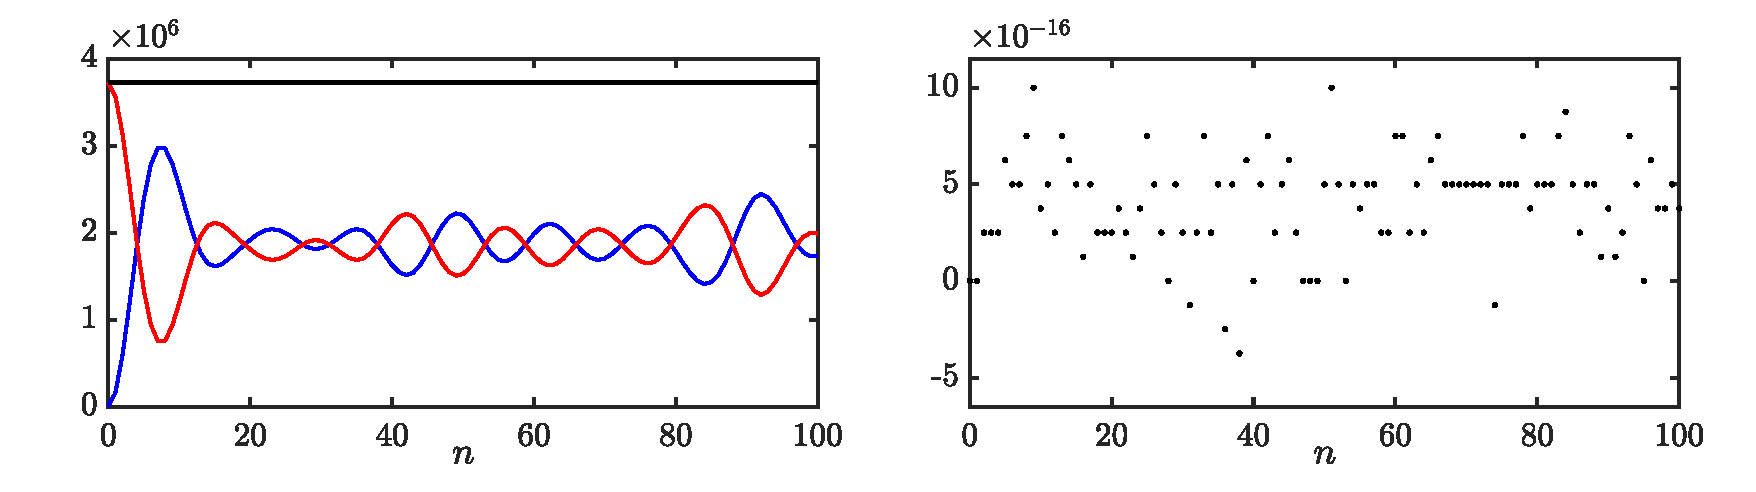
\includegraphics[width=\textwidth]{figures/resonators/2d/energy2DWave.eps}
        };
    
        \node[] (he) at (0.2,0.5) {\small $\mathfrak{h}_\text{e}$};

        \node[] (h) at (-5.75, 1) {\small $\mathfrak{h}$};
        \node[] (v) at (-5.75, 0.5) {\small $\color{red}\mathfrak{v}$};
        \node[] (t) at (-5.75, 0) {\small $\color{blue}\mathfrak{t}$};
      \end{tikzpicture}
      \caption{The kinetic (blue), potential (red), and total (black) energy of an implementation of the 2D wave equation are plotted in the left panel. The right panel shows the normalised energy (according to Eq. \eqref{eq:normalisedEnergy}) and shows that the deviation of the energy is within machine precision. \label{fig:energy2Dwave}}
\end{figure}

\subsection{Modal analysis in 2D}
Given that the state vector is stacked as described in Section \ref{sec:2DwaveImplementation} and the update equation is written in matrix form as in Eq. \eqref{eq:matrixUpdate2Dwave}, performing a modal analysis on a 2D system does not differ from a 1D system and follows the same process presented in Section \ref{sec:modalAnalysis}.

Inserting a test solution of $\uStack^n = z^n\boldPhi$ into the matrix form of the 2D wave equation in Eq. \eqref{eq:matrixUpdate2Dwave} yields the following characteristic equation
\begin{equation}
   \left(z - 2 + z^{-1}\right)\boldPhi = c^2k^2\DDeltamat\boldPhi.
\end{equation}
The $p$\th modal frequency can then be obtained by finding the roots of 
\begin{equation}
    z_p + \left(-2 - c^2k^2\text{eig}_p(\DDeltamat)\right) + z_p^{-1} = 0,
\end{equation}
which, using test solution $z_p = e^{j\omega_p k}$ for (angular) frequency $\omega_p$, can be shown to be 
\begin{equation}\label{eq:2DWaveModes}
    f_p = \frac{1}{\pi k}\sin^{-1}\left(\frac{ck}{2}\sqrt{-\text{eig}_p(\DDeltamat)}\right).
\end{equation}
Notice the similarity to the equation for the modal frequencies of the 1D wave equation in Eq. \eqref{eq:1DWaveModes}. Again, the number of modes is equal to the number of moving grid points in the system. 

See Figure \ref{fig:modalFreqs2Dwave} for the result of a modal analysis of the 2D wave equation. One can observe that the modes do not follow a linear pattern as opposed to those of the 1D wave equation shown in Figure \ref{fig:modalFreqs1Dwave}. This confirms the inharmonic behaviour of the 2D wave equation discussed \ref{sec:2DwaveImplementation}. 
\begin{figure}[h]
    \centering
    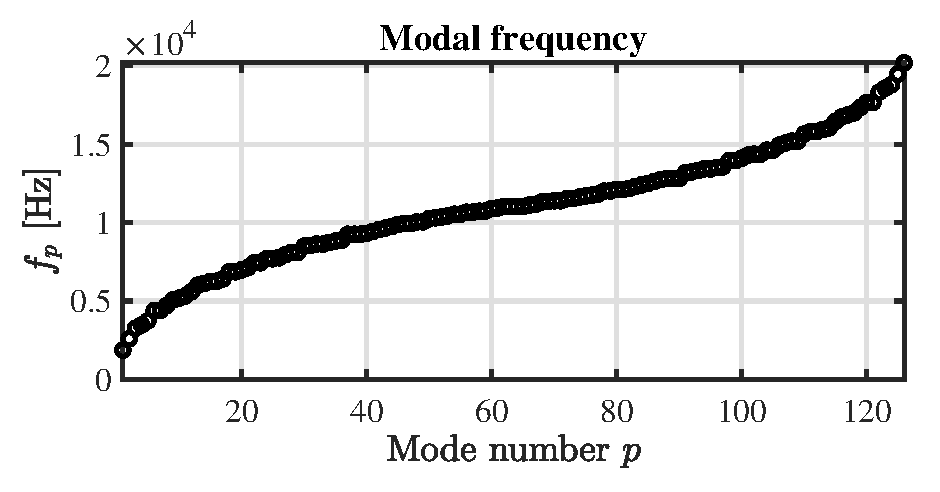
\includegraphics[width = 0.6\textwidth]{figures/resonators/2d/modes2Dwave.eps}
    \caption{Modal frequencies of the 2D wave equation with $L_x = 1.5$ m, $L_y = 1$ m and $c\approx 3118$ m/s, such that $\lambda = 1/\sqrt{2}$ according to Eq. \eqref{eq:CFL2D}. \label{fig:modalFreqs2Dwave}}
\end{figure}
\subsubsection{Modal shapes}
Using the line of code in Appendix \ref{sec:eigenValueProblems} and the \texttt{reshape} function, the modal shapes of the system can also be obtained. Figure \ref{fig:modalShapes2D} shows the six lowest-frequency modes of the 2D wave equation with $L_x = 1.5$ m and $L_y = 1$ m. The mode number $(x,y)$ corresponds to the modal number in the $x$ and $y$ direction.

\begin{figure}[h]
    \centering
    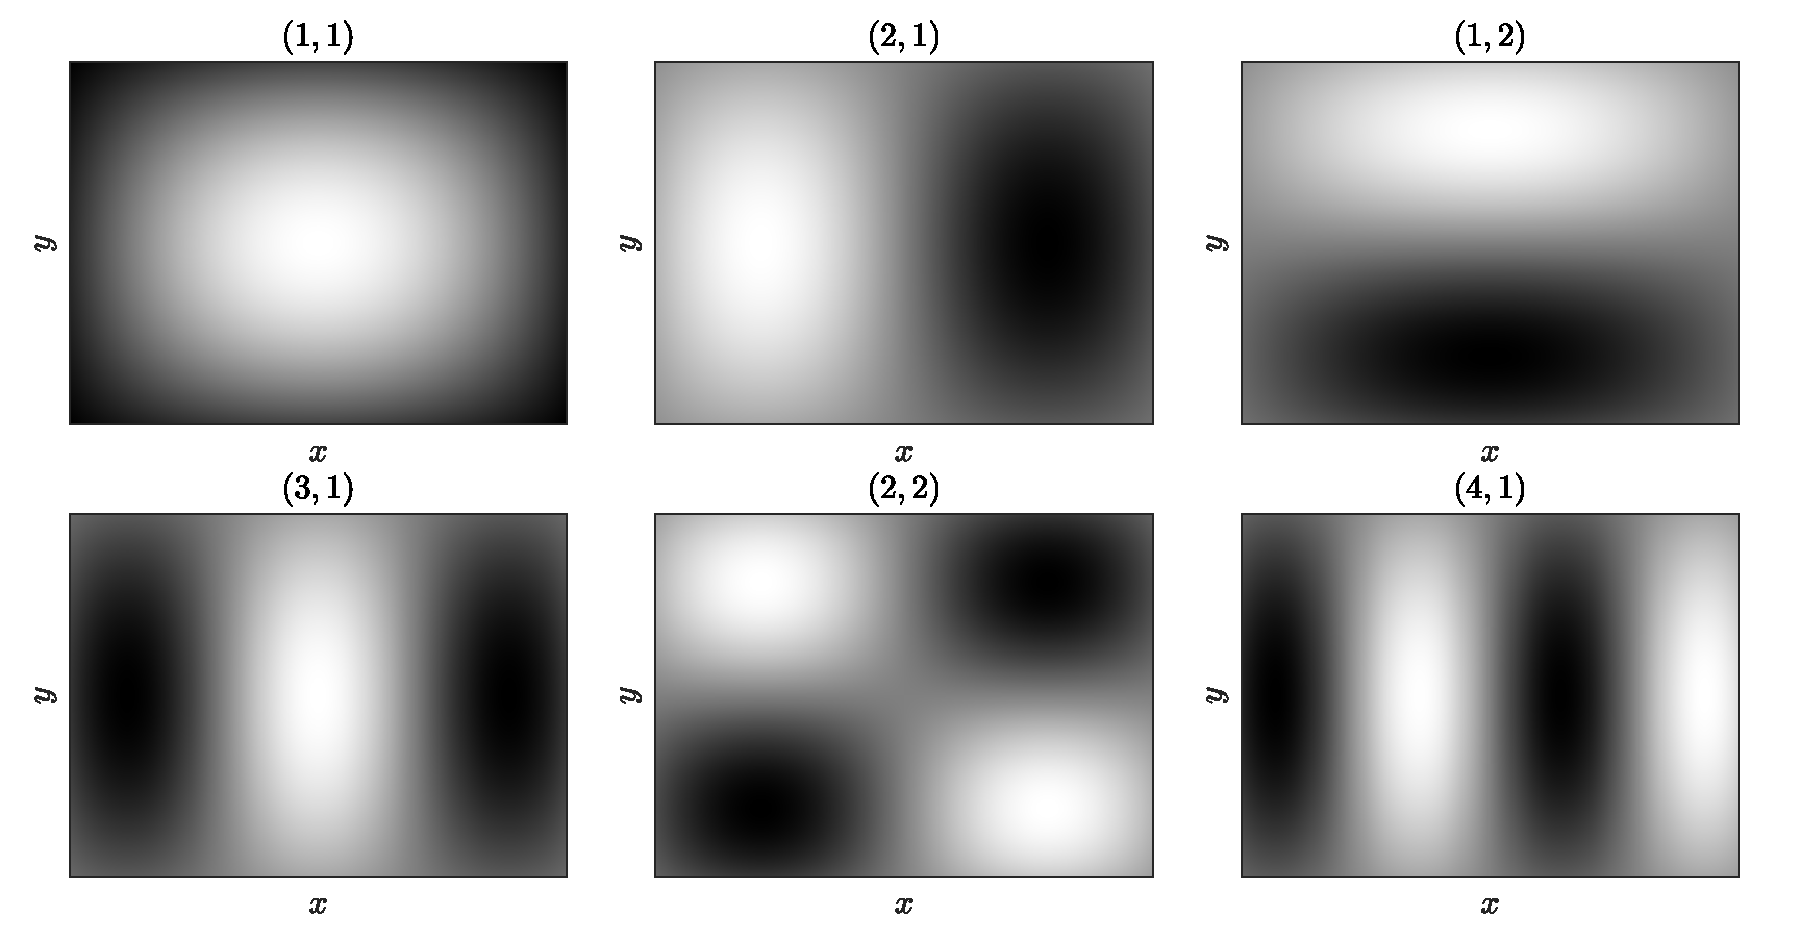
\includegraphics[width=\textwidth]{figures/resonators/2d/modalShapes.eps}
    \caption{The first six (lowest-frequency) modal shapes of 2D wave equation with $L_x = 1.5$ m and $L_y = 1$ m.%and rho = 7850; H =  0.0005; T = 1000000;
    \label{fig:modalShapes2D}}
\end{figure}

\section{The thin plate}\label{sec:thinPlate}
The thin plate, also known as the Kirchhoff model \cite{Kirchhoff1968}, differs from the 2D wave equation in that its restoring force is solely due to stiffness rather than tension. Like for the stiffness term in the stiff string (see Chapter \ref{ch:stiffString}), this causes frequency dispersion, and exhibits interesting timbres. 

The plate model is quite versatile and can be used to model a plate reverb \cite{DAFxChapter} as well as simplified instrument bodies, as done in \citeP[A], \citeP[B], \citeP[D] and \citeP[E]. This section presents the thin plate PDE and FD scheme, after which it will be subjected to the various analysis techniques extended to 2D in the previous section.

\subsection{Continuous time}
Consider a rectangular thin plate with side lengths $L_x$ and $L_y$ (both in m) and its transverse displacement described by $u=u(x,y,t)$ (in m). The system is defined for $(x,y)\in \D$ where 2D domain $\D = [0, L_x]\times [0, L_y]$. Using the biharmonic operator introduced in Eq. \eqref{eq:biharmonic}, the PDE for the thin plate can be defined as \cite{Kirchhoff1968}
\begin{equation}\label{eq:platePDENoLosses}
    \rho H \ptt u = -D\Delta\Delta u,
\end{equation}
where $D = EH^3/12(1-\nu^2)$ is a stiffness coefficient (in kg $\cdot$ m$^2\cdot$s$^{-2}$) parametrised by Young's Modulus $E$ (in Pa), thickness $H$ (in m) and the dimensionless Poisson's ratio $\nu$. Although Eq. \eqref{eq:platePDENoLosses} does not hold for thick plates and only accounts for low-amplitude vibration (as it is linear), these properties can be assumed in musical instrument simulations, making this model sufficient in this work. 

Adding losses to Eq. \eqref{eq:platePDENoLosses} yields
%
\begin{equation}\label{eq:platePDE}
    \rho H \ptt u = -D\Delta\Delta u - 2\sz \rho H \pt u + 2 \so\rho H  \pt \Delta u
\end{equation}
where, as in the case of the stiff string in Eq. \eqref{eq:stiffStringPDE}, $\sz$ and $\so$ are the frequency independent (in s$^{-1}$) and frequency dependent damping coefficient (in m$^2$/s) respectively.\todo{check hyphens after `frequency'}

\subsubsection{Boundary conditions}
Similar to the stiff string, clamped and simply supported boundary conditions can be defined as
\begin{subequations}\label{eq:boundaryCondThinPlate}
    \begin{align}
        \begin{rightcases}
            u = \px u = 0,\quad \text{if } y=\{0 , L_y\}, \quad \forall x\\
            u = \py u = 0,\quad \text{if } x=\{0 , L_x\},\quad \forall y
        \end{rightcases}
     \quad &\text{(Clamped)},\label{eq:contClamped2D}\\
     \begin{rightcases}
        u = \pxx u = 0,\quad \text{if } y=\{0 , L_y\}, \quad \forall x\\
        u = \pyy u = 0,\quad \text{if } x=\{0 , L_x\},\quad \forall y
    \end{rightcases}\quad &\text{(Simply supported)}.\label{eq:contSimplySupported2D}
    \end{align}
\end{subequations}
 Naturally, a free condition can be added too, but is much less trivial. As it will not be used in this work, it will not be given here, and the interested reader is instead referred to \cite[Ch. 12]{theBible}. 

\subsection{Discrete time}
Equation \eqref{eq:platePDE} can be discretised to the following FD scheme:
\begin{equation}\label{eq:thinPlateFDS}
    \rho H \dtt \ulmn = - D \dDelta\dDelta\ulmn - 2\sz \rho H \dtd \ulmn + 2 \so \rho H \dtm \dDelta\ulmn
\end{equation}
where $l\in\{0, \hdots, N_x\}$ and $m\in\{0, \hdots, N_y\}$. Like for the stiff string FD scheme in Eq. \eqref{eq:stiffStringFDS}, the backwards difference operator is used for the frequency-dependent damping term to yield an explicit scheme. A more compact way to write this scheme is after a division by $\rho H$ which yields
\begin{equation}\label{eq:thinPlateFDSCompact}
    \dtt \ulmn = - \kappa^2\dDelta\dDelta\ulmn - 2\sz\dtd \ulmn + 2 \so \dtm \dDelta\ulmn
\end{equation}
with
\begin{equation}\label{eq:kappaDef}
     \kappa = \sqrt{\frac{D}{\rho H}}\ .
\end{equation}
Using the expansion of the discrete biharmonic operator in Eq. \eqref{eq:discreteBiharmonic}, Eq. \eqref{eq:thinPlateFDSCompact} can be expanded and solved for $\ulm^{n+1}$ according to
\begin{equation}\label{eq:plateUpdate}
    \begin{aligned}
    \ulm^{n+1} =&\ (2-20\mu^2 - 4S)\ulmn \\
    &\ \ \ +(8\mu^2 + S)(u_{l+1, m}^n + u_{l-1, m}^n+u_{l, m+1}^n+u_{l, m-1}^n)\\
    &\ \ \ -2\mu^2(u_{l+1, m+1}^n + u_{l-1, m+1}^n+u_{l+1, m-1}^n+u_{l-1, m-1}^n)\\
    &\ \ \ -\mu^2(u_{l+2, m}^n + u_{l-2, m}^n+u_{l, m+2}^n+u_{l, m-2}^n),\\
    &\ \ \ + (\sz k  - 1 + 4S) \ulm^{n-1}\\
    &\ \ \ - S (u_{l+1, m}^{n-1} + u_{l-1, m}^{n-1}+u_{l, m+1}^{n-1}+u_{l, m-1}^{n-1})
    \end{aligned}
\end{equation}
where 
\begin{equation}
    \mu = \frac{\kappa k}{h^2}
\end{equation}
and $S = 2\so k / h^2$ for compactness. See Figure \ref{fig:plateStencil} for the stencil of this scheme.
\def\figSpacing{0.01\textwidth}
\def\figWidth{0.49\textwidth}
\begin{figure}[t]
    \centering
    \subfloat[Full stencil.\label{fig:fullStencilPlate}]{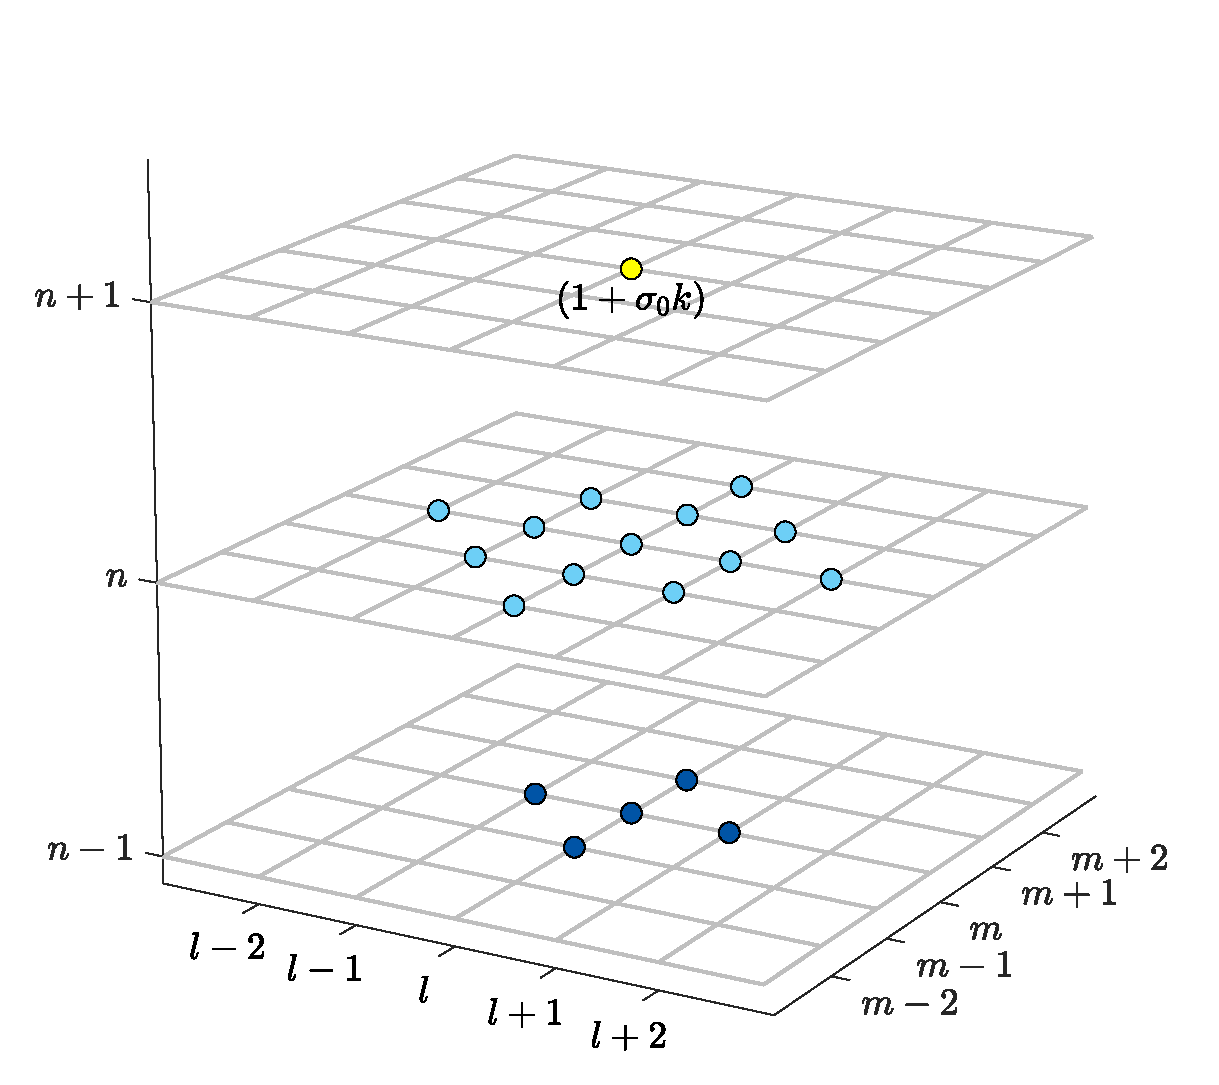
\includegraphics[width=\figWidth]{figures/resonators/2d/fullPlate.eps}}\\
    \subfloat[Stencil of $u_{l,m}^n$. \label{fig:curStencilPlate}]{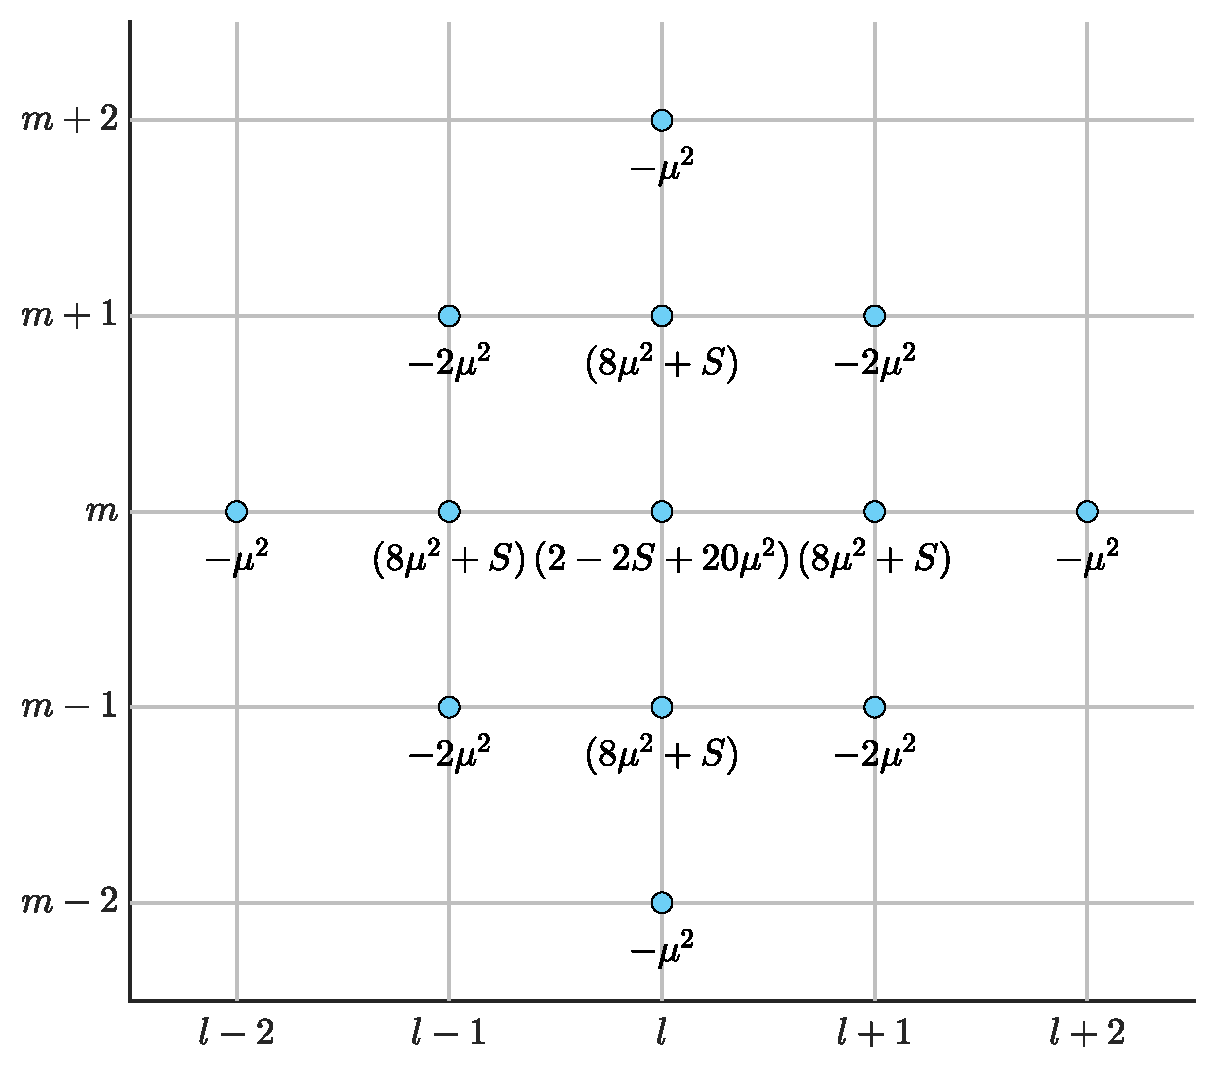
\includegraphics[width=\figWidth]{figures/resonators/2d/curPlateStencil.eps}}\hspace{\figSpacing}
    \subfloat[Stencil of $u_{l,m}^{n-1}$.\label{fig:prevStencilPlate}]{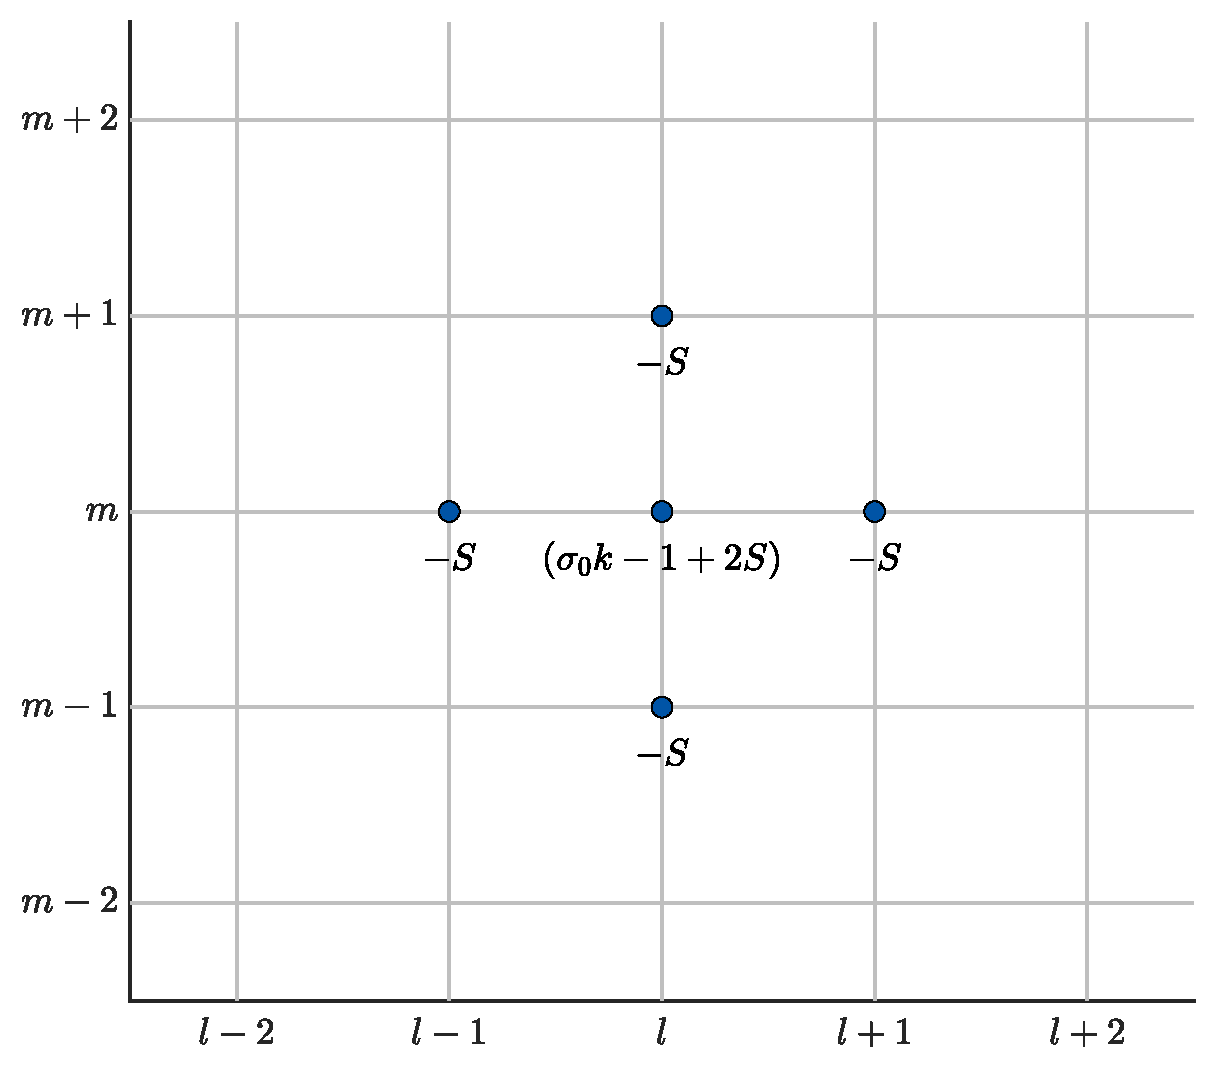
\includegraphics[width=\figWidth]{figures/resonators/2d/prevPlateStencil.eps}}
    \caption{The stencil of the plate with coefficients corresponding to those in update equation \eqref{eq:plateUpdate}. (a) A full overview of the stencil. (b) The current time-step $n$ highlighted. (c) The previous time-step $n-1$ highlighted. \label{fig:plateStencil}}
\end{figure}
%
The stability condition of the scheme can be shown to be
\begin{equation}\label{eq:stabilityPlate}
    h \geq 2\sqrt{k\bigg(\sigma_1 + \sqrt{\kappa^2+ \sigma_1^2}\bigg)},
\end{equation}
and will be derived in Section \ref{sec:stabilityThinPlate}.

\subsubsection{Discrete boundary conditions}
The boundary conditions shown in Eq. \eqref{eq:boundaryCondThinPlate} can be discretised to 
\begin{subequations}\label{eq:boundaryCondThinPlateDisc}
    \begin{align}
        \begin{rightcases}
            \begin{aligned}
                \ulmn = \dxp \ulmn = 0\quad &\text{if } m=0 \ && \forall l\\
                \ulmn = \dxm \ulmn = 0\quad &\text{if } m=N_y \ && \forall l\\
                \ulmn = \dyp \ulmn = 0\quad &\text{if } l=0 \ && \forall m\\
                \ulmn = \dym \ulmn = 0\quad &\text{if } l=N_x \ && \forall m
            \end{aligned}
        \end{rightcases}
     \quad &\text{(Clamped)},\label{eq:discClamped2D}\\
     \begin{rightcases}
        \begin{aligned}
            \ulmn = \dxx \ulmn = 0\quad &\text{if } m=\{0 , N_y\} \ &&\forall l\\
            \ulmn = \dyy \ulmn = 0\quad &\text{if } l=\{0 , N_x\}\ &&\forall m
        \end{aligned}
    \end{rightcases}\quad &\text{(Simply supported)}.\label{eq:discSimplySupported2D}
    \end{align}
\end{subequations}
The clamped condition can be implemented by simply reducing the discrete range of operation to $l = \{2, \hdots, N_x-2\}$ and $m = \{2, \hdots, N_y-2\}$. For the simply supported case, the range of operation reduces to $l = \{1, \hdots, N_x-1\}$ and $m = \{1, \hdots, N_y-1\}$, and similar to the simply supported stiff string described in Section \ref{sec:stiffStringBoundaryConditions}, the virtual grid points needed for this condition become
\begin{align*}
    u_{-1, m}^n = -u_{1, m}^n &\qaq u_{N_x+1, m}^n = -u_{N_x-1, m}^n\quad\forall m,\\
    u_{l, -1}^n = -u_{l, -1}^n &\qaq u_{l, N_y+1}^n = -u_{l, N_y-1}^n\qquad \forall l.
\end{align*}

\subsection{Matrix form and output}
Similar to the implementation of the 2D wave equation in Section \ref{sec:2DwaveImplementation}, one can use a stacked state vector. If simply supported boundary conditions are used, one can easily obtain a matrix form of the $\dDelta\dDelta$ operator by multiplying two $\DDeltamat$ matrices presented in Eq. \eqref{eq:DDeltaMatrix} to get $\DDeltaDelta = \DDeltamat\DDeltamat$.

Using a stacked form of the state as described in Eq. \eqref{eq:stackedState} the scheme in Eq. \eqref{eq:thinPlateFDSCompact} in matrix form is     
\begin{equation}\label{eq:matrixFormThinPlate}
    A\uStack^{n+1} = \B\uStack^n + \C\uStack^{n-1},
\end{equation}
where
\begin{gather*}
    A = (1+\sz k),\quad \B = 2\I - \kappa^2 k^2 \DDeltaDelta + 2 \so k\DDeltamat, \\
    \text{and}\quad \C = -(1-\sz k)\I - 2\so k \DDeltamat,
\end{gather*}
and the identity matrix $\I$ is of the same size as $\DDeltaDelta$ and $\DDeltamat$.

As a starting point for implementation, possible parameters are given in Table \ref{tab:thinPlateParams}. Figure \ref{fig:thinPlatePropagation} shows the wave propagation of a thin plate using these parameters, and excited using the same excitation as used for the 2D wave equation in Section \ref{sec:2DwaveImplementation} (a 2D raised cosine at $(x,y) = (0.25L_x, 0.5L_y)$). When compared to Figure \ref{fig:2Dpropagation}, dispersive effects -- where higher-frequency components travel faster than lower-frequency ones -- are apparent due to stiffness.

\begin{table}[h]
    \begin{center}
    \begin{tabular}{|l|c|c|}
        \hline
        Name & Symbol (unit) & Value\\ \hline
        Side length $x$ & $L_x$ (m) & $1.5$\\
        Side length $y$  & $L_y$ (m) & $1$\\
        Material density & $\rho$ (kg/m$^3$) & $7850$\\
        Thickness & $H$ (m) & $5\cdot10^{-3}$\\
        Young's modulus & $E$ (Pa) & $2\cdot10^{11}$\\
        Poisson's ratio & $\nu$ (-)& $0.3$\\
        Freq.-independent damping & $\sz$ (s$^{-1}$) & $1$\\
        Freq.-dependent damping & $\so$ (m$^2$/s) & $0.005$\\\hline
    \end{tabular}
    \caption{Parameters for the thin plate and possible values to use as a starting point for the simulation.\label{tab:thinPlateParams}}
    \end{center}
\end{table}
{\renewcommand{\arraystretch}{1}

Figure \ref{fig:outputThinPlate} shows the time domain and frequency domain output of the thin plate at $(x,y) = (0.15L_x, 0.85 L_y)$.
Compared to the output of the 2D wave equation in Figure \ref{fig:output2DWave}, there are several interesting differences. The amplitude is much lower, waves are closer together and the first wave arrives much earlier, all due to dispersive effects.
\begin{figure}[h]
    \centering
    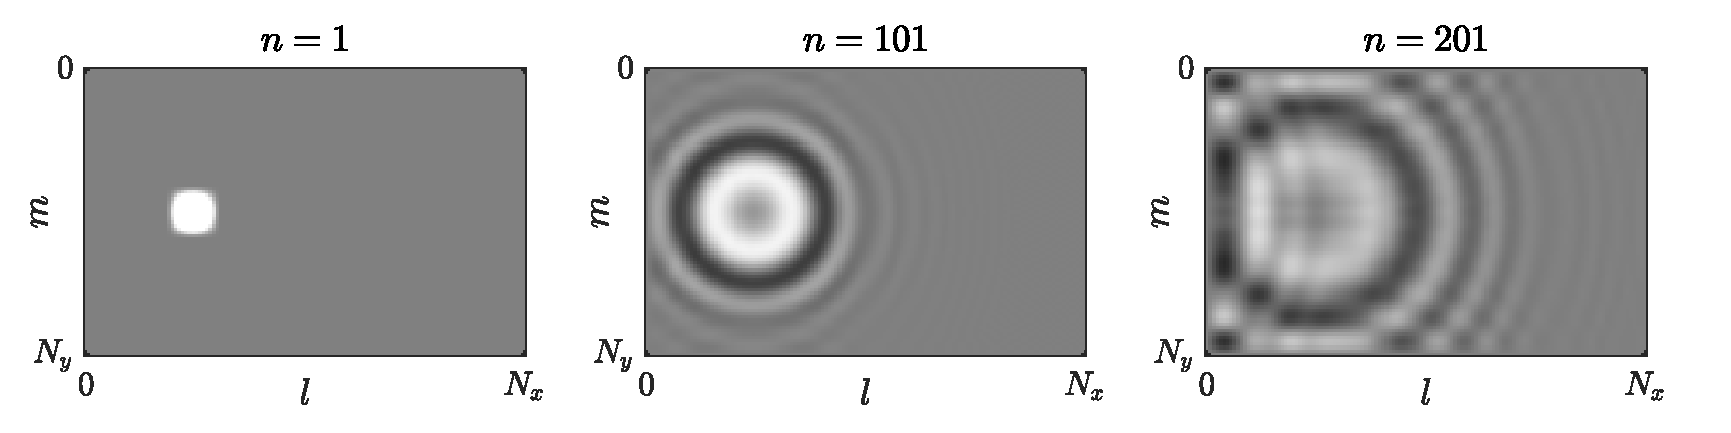
\includegraphics[width = \textwidth]{figures/resonators/2d/thinPlatePropagation.eps}
    \caption{Wave propagation of a thin plate with simply supported boundary conditions and parameters as shown in Table \ref{tab:thinPlateParams}. The system is excited with a 2D raised cosine at $(x,y) = (0.25L_x, 0.5L_y)$ and dispersive effects are apparent.\label{fig:thinPlatePropagation}}
\end{figure}

\begin{figure}[h]
    \centering
    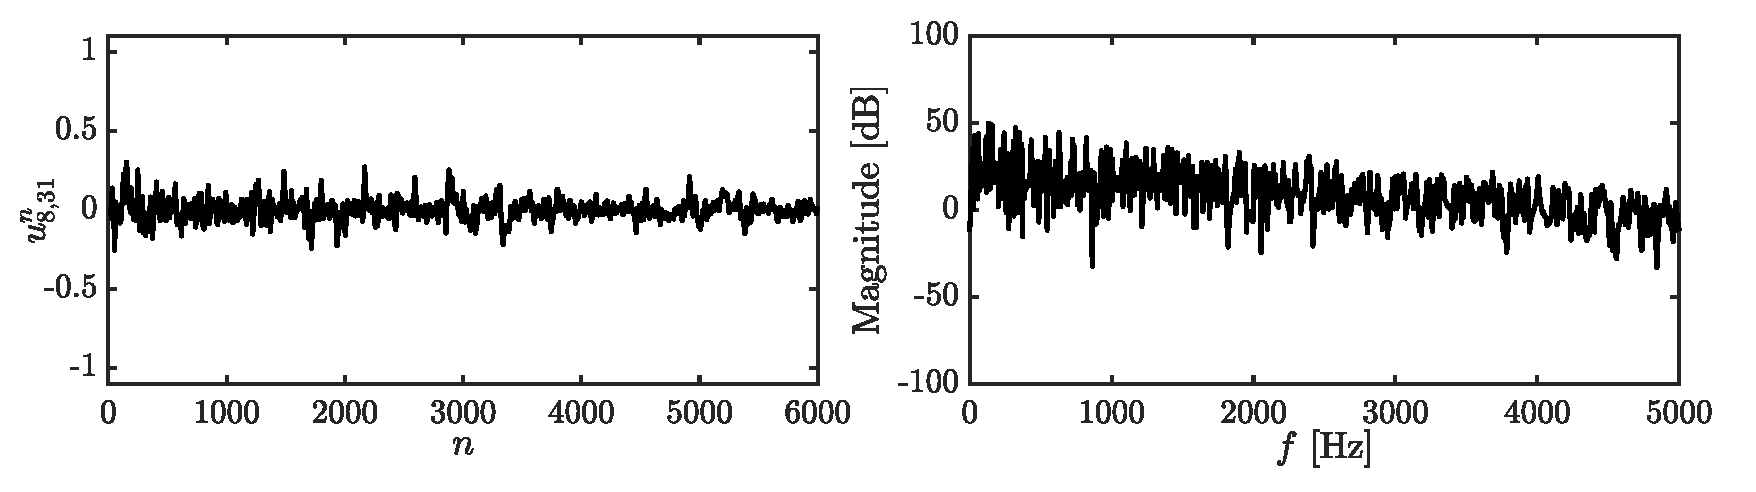
\includegraphics[width=\textwidth]{figures/resonators/2d/outputThinPlate.eps}
    \caption{The output of the thin plate at $(x,y) = (0.15, 0.85)$ corresponding to Figure \ref{fig:thinPlatePropagation}. \label{fig:outputThinPlate}}
\end{figure}\todo{FULL DOC SWEEP: check figure alignment}

\subsection{Frequency domain analysis}\label{sec:stabilityThinPlate}
This section follows the process presented in Section \ref{sec:stabilityAnalysis} with the extensions to 2D shown in \ref{sec:stability2Dwave}.

Using Eqs. \eqref{eq:laplacianAnsatz} and \eqref{eq:biharmonicAnsatz} one can obtain a frequency domain representation of the FD scheme in Eq. \eqref{eq:thinPlateFDSCompact}
and obtain the following characteristic equation
\begin{equation}
    \begin{aligned}
        (1+\sigma_0k)z + &\left(16\mu^2(p_x+p_y)^2 + \frac{8\sigma_1k}{h^2}(p_x+p_y) - 2\right) \\
        &+ \left(1 - \sigma_0k - \frac{8\sigma_1k}{h^2}(p_x+p_y)\right)z^{-1} = 0.
    \end{aligned}
\end{equation}
This can, similar to the damped stiff string in Section \ref{sec:stiffStringStability}, be solved to
\begin{equation*}
    4\mu^2(p_x+p_y)^2 + \frac{4\sigma_1k}{h^2}(p_x+p_y) \leq 1.
\end{equation*}
Recalling the definitions $p_x$ and $p_y$ in Eq. \eqref{eq:pxpy}, and given the fact that these are bounded by 1, the following can be written
\begin{gather*}
    4\mu^2(1+1)^2 + \frac{4\sigma_1k}{h^2}(1+1) \leq 1\\
    16\mu^2 + \frac{8\sigma_1k}{h^2} \leq 1.
\end{gather*}
Finally, recalling the definition for $\kappa$ in Eq. \eqref{eq:kappaDef} solving for $h$ yields
\begin{align}
    &1 \geq \frac{16\kappa^2k^2}{h^4} + \frac{8\sigma_1k}{h^2}\nonumber,\\
    &h^4 - 8\sigma_1kh^2 - 16\kappa^2k^2 \geq 0\nonumber,\\
    &h \geq \sqrt{\frac{8\sigma_1k +\sqrt{(8\sigma_1k)^2 + 64\kappa^2k^2}}{2}}\nonumber,\\
    &h\geq \sqrt{\frac{8\sigma_1k+8\sqrt{\sigma_1^2k^2+\kappa^2k^2}}{2}}\nonumber,\\
    &h \geq 2\sqrt{k\left(\sigma_1 + \sqrt{\sigma_1^2 + \kappa^2}\right)},
\end{align}
which is the stability condition given in Eq. \eqref{eq:stabilityPlate}.

\subsection{Energy analysis}\label{sec:energyAnalysisThinPlate}
Using the steps described in Section \ref{sec:energyAnalysis} with the extensions to 2D presented in Section \ref{sec:energyAnalysis2DWave}, one can obtain the total energy of the FD scheme in Eq. \eqref{eq:thinPlateFDSCompact}.
\subsubsection{Step 1: Obtain $\dtp \h$}
To obtain the rate of change of the total energy, one can take an inner product of the scheme in Eq. \eqref{eq:thinPlateFDSCompact} with $(\dtd \ulmn)$ over discrete (2D) domain $d = \{0, \hdots, N_x\}\times \{0, \hdots, N_y\}$ to get
\begin{equation}\label{eq:rOCthinPlate}
    \begin{aligned}
        \dtp \h =&\ \rho H \langle \dtd \ulmn, \dtt \ulmn \rangle_d + D \langle \dtd \ulmn, \dDelta\dDelta \ulmn \rangle_d\\
        & + 2\sz\rho H\langle \dtd \ulmn, \dtd \ulmn \rangle_d - 2\so \rho H\langle \dtd \ulmn, \dtm \dDelta \ulmn \rangle_d = 0.
    \end{aligned}
\end{equation}

\subsubsection{Step 2: Identify energy types and isolate $\dtp$}
Due to the damping present in the system and because the system is distributed in space, the energy balance will be of the following form
\begin{equation*}
    \dtp \h = \b-\q, 
\end{equation*}
with boundary term $\b$ and damping term
\begin{equation}\label{eq:dampingTermThinPlate}
    \mathfrak{q} = 2\sz \rho H \lVert\dtd\ulmn\rVert_d^2 - 2 \so \rho H \langle \dtd \ulmn, \dtm \dDelta\ulmn \rangle_d.
\end{equation}
Expanding the stiffness term in Eq. \eqref{eq:rOCthinPlate} to
\begin{align*}
    &\ D\langle \dtd \ulmn, (\dxx + \dyy)\dDelta \ulmn \rangle_d\\
    \Longleftrightarrow\ \ &\ D\left(\langle \dtd \ulmn, \dxx\dDelta \ulmn \rangle_d + \langle \dtd \ulmn, \dyy\dDelta \ulmn \rangle_d\right),
\end{align*} 
one can perform summation by parts twice, using Eq. \eqref{eq:summationByPartsTwiceReduced} for both terms to get
\begin{equation*}
    D\left(\langle \dtd \dxx\ulmn, \dDelta \ulmn \rangle_{\domXredBoth} + \langle \dtd\dyy \ulmn, \dDelta \ulmn \rangle_{\domYredBoth}\right) + \b.
\end{equation*}
The definitions for the reduced domains can be found in Eqs. \eqref{eq:reduced2Ddoms}. Finally, as the boundaries are always $0$ due to the boundary conditions in Eq. \eqref{eq:boundaryCondThinPlateDisc}, $\domXredBoth$ and $\domYredBoth$ can be further reduced to $\domRedBoth$ and the terms can be combined as \SWcomment[check with stefan]\todo{FULL DOC SWEEP: check for SWcomments}
\begin{equation*}
    D\langle \dtd\dDelta\ulmn, \dDelta \ulmn \rangle_{\domRedBoth} + \b ,
\end{equation*}
and using identities \eqref{eq:prodIdentity1} and \eqref{eq:prodIdentity2} a definition for the total energy can be found:
\begin{equation}\label{eq:energyBalanceThinPlate}
    \begin{gathered}
        \h = \t + \v, \qwiq \t = \frac{\rho H}{2} \left\lVert\delta_{t-}\ulmn\right\rVert_{d}^2 \quad \text{and} \\
        \v = \frac{D}{2}\langle\dDelta \ulmn, e_{t-}\dDelta \ulmn\rangle_{\overline{\underline{d}}}\ .
    \end{gathered}
\end{equation}
The definition of the boundary term $\b$ will not be given here, but can be shown to vanish under the boundary conditions given in Eq. \eqref{eq:boundaryCondThinPlateDisc} \cite{theBible}.

\subsubsection{Step 3: Check units}
As $\t$ is identical to its definition in Eq. \eqref{eq:energyBalance2DWave}, only the units for $\v$ will be checked here. Recalling that $D = EH^3 / 12(1-\nu^2)$, which in units is kg$\cdot$ m$^2\cdot$s$^{-2}$, yields
\begin{align*}
    \v = \frac{D}{2}\langle\dDelta \ulmn, e_{t-}\dDelta \ulmn\rangle_{\overline{\underline{d}}} \
    \overset{\text{in units}}{\xrightarrow{\hspace*{1cm}}} \ & \text{kg} \cdot \text{m}^2\cdot\text{s}^{-2}\cdot\text{m}^2\cdot(\text{m}^{-2}\cdot\text{m})\cdot(\text{m}^{-2}\cdot\text{m})\nonumber \\
    = \ &\text{kg}\cdot\text{m}^2\cdot\text{s}^{-2}
\end{align*}
and shows that $\v$ indeed has the correct units. 

\subsubsection{Step 4: Implementation}
Figure \ref{fig:energyThinPlate} shows the energetic output of an implementation of the thin plate and shows that the energy is conserved.
\begin{figure}[h]
    \centering
    \begin{tikzpicture}[->,node distance=3cm,
        thick,main node/.style={circle,draw}]
    
        \node[] (image) at (0,0) {
        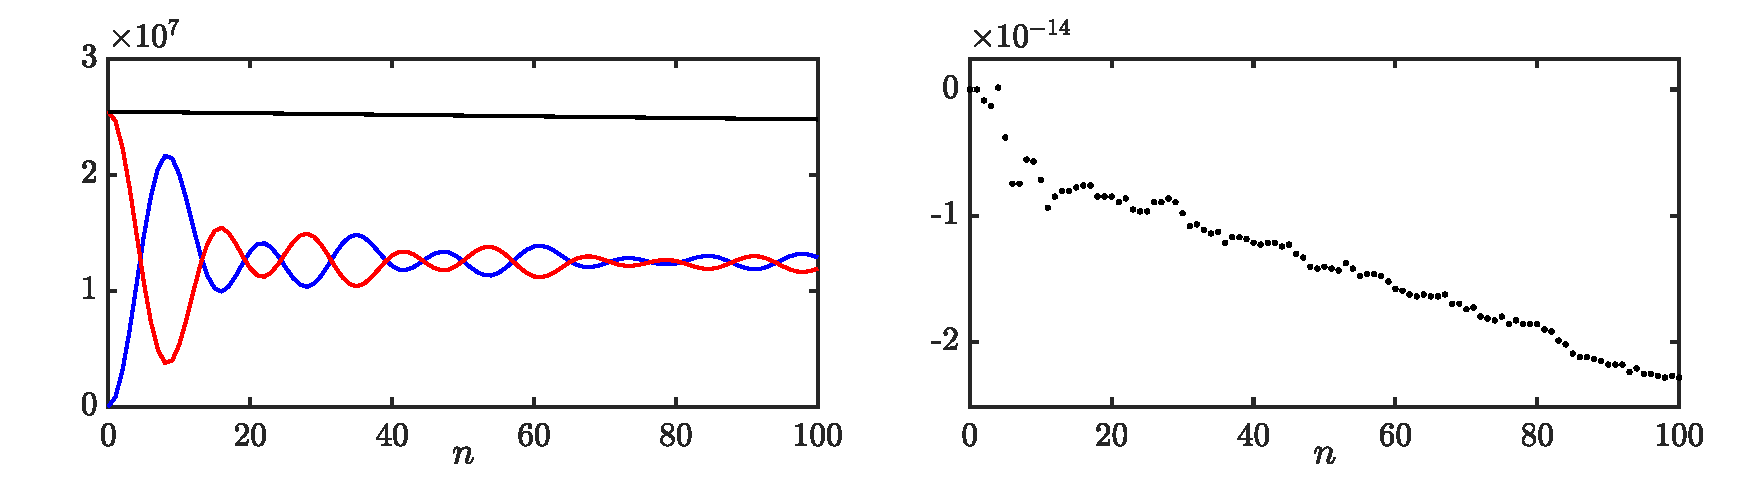
\includegraphics[width=\textwidth]{figures/resonators/2d/energyThinPlate.eps}
        };
    
        \node[] (he) at (0.2,0.5) {\small $\mathfrak{h}_\text{e}$};

        \node[] (h) at (-5.75, 1) {\small $\mathfrak{h}$};
        \node[] (v) at (-5.75, 0.5) {\small $\color{red}\mathfrak{v}$};
        \node[] (t) at (-5.75, 0) {\small $\color{blue}\mathfrak{t}$};
      \end{tikzpicture}
      \caption{The kinetic (blue), potential (red), and total (black) energy of an implementation of the thin plate are plotted in the left panel. Notice that the damping present in the system causes $\h$ to decrease. The right panel shows the normalised energy (according to Eq. \eqref{eq:normalisedEnergyDamping}) and shows that the deviation of the energy is within machine precision. \label{fig:energyThinPlate}}
\end{figure}

\subsection{Modal analysis}
Using the matrix form in Eq. \eqref{eq:matrixFormThinPlate}, a modal analysis of the system can be performed using a one-step form described in Section \ref{sec:oneStepForm}.

Figure \ref{fig:thinPlateModes} shows the results of the analysis with parameter values as listed in Table \ref{tab:thinPlateParams}. Although the modal frequencies follow a similar pattern to those of the 2D wave equation in Figure \ref{fig:modalShapes2D}, the pattern is slightly more exponential like the stiff string in Figure \ref{fig:modesStiffString}.\SWcomment[not really sure what to say here honestly] 

\begin{figure}[h]
    \centering
    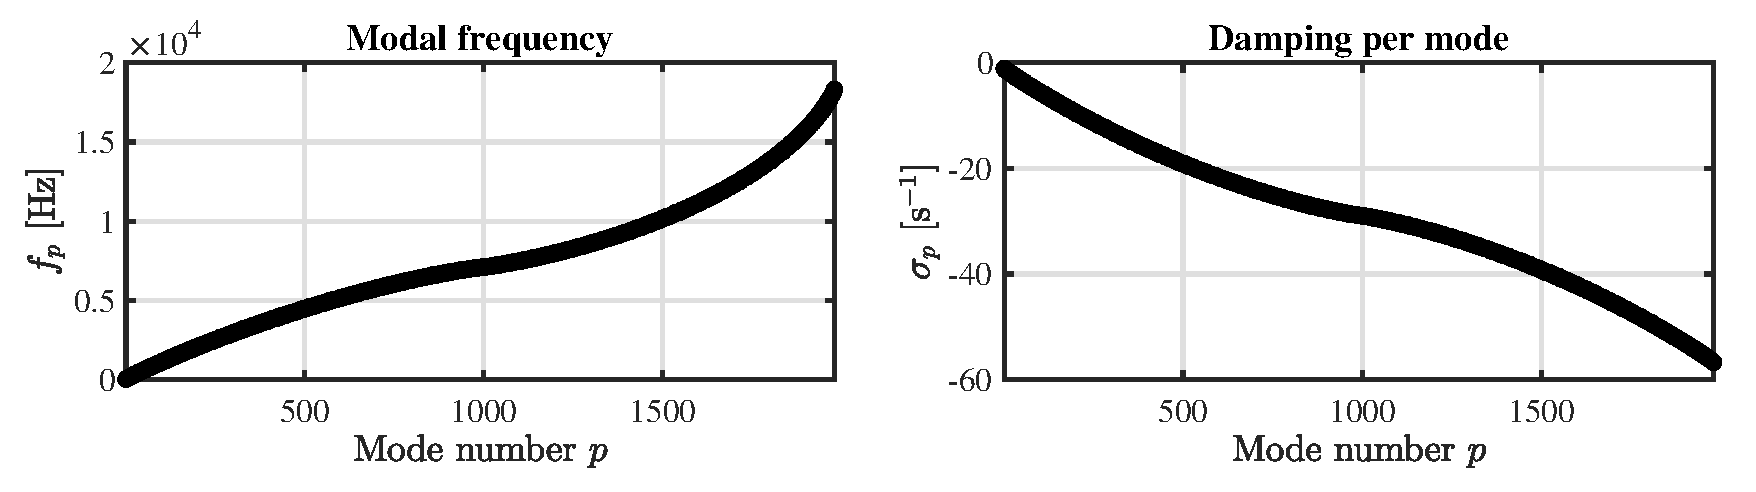
\includegraphics[width=\textwidth]{figures/resonators/2d/thinPlateModes.eps}
    \caption{The result of a modal analysis of the thin plate using the parameters in Table \ref{tab:thinPlateParams}. Notice that the damping is plotted against modal frequency rather than mode number. \label{fig:thinPlateModes}}
\end{figure}

\section{The stiff membrane}
The term \textit{stiff membrane} first appeared in \cite{Fletcher1998}\todo{true?} and is essentially a 2D version of the stiff string. It can be used to model membranes with dispersive effects or provide tension control for thin plates. In this work, the stiff membrane has only been used in paper \citeP[F] to model a drum membrane. 

Similar to previous sections, this section will provide the continuous-time and discrete-time equations of the model. Only a frequency domain analysis will be given, as energy and modal analyses are too similar to those previously presented.

\subsection{Continuous time}
The PDE for a stiff membrane can be obtained as a combination of the 2D wave equation in Eq. \eqref{eq:2DwavePDE} and the thin plate in Eq. \eqref{eq:platePDENoLosses}. Adding losses as in Eq. \eqref{eq:platePDE} yields the following PDE
\begin{equation}\label{eq:stiffMembranePDE}
    \rho H \ptt u = T\Delta u - D
    \Delta\Delta u- 2\sz \rho H \pt u + 2 \so\rho H  \pt \Delta u,
\end{equation}
where the parameters are identical to those in Eqs. \eqref{eq:2DwavePDE} and \eqref{eq:platePDE}.

\subsection{Discrete time}
Using familiar operators, Eq. \eqref{eq:stiffMembranePDE} can be discretised to 
\begin{equation}\label{eq:stiffMembraneFDS}
    \rho H \dtt \ulmn = T\dDelta\ulmn- D \dDelta\dDelta\ulmn - 2\sz \rho H \dtd \ulmn + 2 \so \rho H \dtm \dDelta\ulmn,
\end{equation}
or, using a more compact form after division by $\rho H$, to
\begin{equation}\label{eq:stiffMembraneFDScompact}
    \dtt \ulmn = c^2\dDelta\ulmn- \kappa^2 \dDelta\dDelta\ulmn - 2\sz \dtd \ulmn + 2 \so \dtm \dDelta\ulmn,
\end{equation}
where $c = \sqrt{T / \rho H}$ and $\kappa = \sqrt{D / \rho H}$.

The update equation can then be obtained using the expansions of the Laplacian and biharmonic operators in Eqs. \eqref{eq:discreteLaplacian} and \eqref{eq:discreteBiharmonic} respectively, to get
\begin{equation}\label{eq:stiffMembraneUpdate}
    \begin{aligned}
    \ulm^{n+1} =&\ (2 - 4\lambda^2 - 20\mu^2 - 4S)\ulmn \\
    &\ \ \ +(\lambda^2 + 8\mu^2 + S)(u_{l+1, m}^n + u_{l-1, m}^n+u_{l, m+1}^n+u_{l, m-1}^n)\\
    &\ \ \ -2\mu^2(u_{l+1, m+1}^n + u_{l-1, m+1}^n+u_{l+1, m-1}^n+u_{l-1, m-1}^n)\\
    &\ \ \ -\mu^2(u_{l+2, m}^n + u_{l-2, m}^n+u_{l, m+2}^n+u_{l, m-2}^n),\\
    &\ \ \ + (\sz k  - 1 + 4S) \ulm^{n-1}\\
    &\ \ \ - S (u_{l+1, m}^{n-1} + u_{l-1, m}^{n-1}+u_{l, m+1}^{n-1}+u_{l, m-1}^{n-1})
    \end{aligned}
\end{equation}
where 
\begin{equation}\label{eq:lambdaMuStiffMembrane}
    \lambda = \frac{c k}{h}\qaq \mu = \frac{\kappa k}{h^2}
\end{equation}
and again, $S = 2\so k / h^2$ for compactness. The stability condition for this scheme will be given in Section \ref{sec:stabilityStiffMembrane}.

\subsection{Implementation}
Writing Eq. \eqref{eq:stiffMembraneFDScompact} in matrix form, yields 
\begin{equation}
    A\uStack^{n+1} = \B\uStack^n + \C\uStack^{n-1},
\end{equation}
with
\begin{gather*}
    A = (1+\sz k),\quad \B = 2\I + c^2k^2 \DDeltamat - \kappa^2 k^2 \DDeltaDelta + 2 \so k\DDeltamat, \\
    \text{and}\quad \C = -(1-\sz k)\I - 2\so k \DDeltamat.
\end{gather*}
Notice that the only difference with Eq. \eqref{eq:matrixFormThinPlate} is the addition of the wave speed term in the definition of the $\B$ matrix. 

\subsection{Frequency domain analysis}\label{sec:stabilityStiffMembrane}
Following familiar techniques from Sections \ref{sec:oneStepForm} and \ref{sec:stability2Dwave}, the characteristic equation of the FD scheme in Eq. \eqref{eq:stiffMembraneFDScompact} can be obtained:
\begin{equation}
    \begin{aligned}
        (1+\sigma_0k)z + &\left(4\lambda^2 (p_x+p_y) + 16\mu^2(p_x+p_y)^2 + \frac{8\sigma_1k}{h^2}(p_x+p_y) - 2\right) \\
        &+ \left(1 - \sigma_0k - \frac{8\sigma_1k}{h^2}(p_x+p_y)\right)z^{-1} = 0.
    \end{aligned}
\end{equation}
Similar to the stiff string in Section \ref{sec:stiffStringStability} and the thin plate in Section \ref{sec:stabilityThinPlate}, this can be solved to 
\begin{equation*}
    \lambda^2(p_x+p_y) + 4\mu^2(p_x+p_y)^2 + \frac{4\sigma_1k}{h^2}(p_x+p_y) \leq 1,
\end{equation*}
and recalling that $p_x$ and $p_y$ are bounded by $1$, yields
\begin{align*}
    \lambda^2(1 + 1) + 4\mu^2(1+1)^2 + \frac{4\sigma_1k}{h^2}(1+1) &\leq 1,\\
    2\lambda^2 + 16\mu^2 + \frac{8\sigma_1k}{h^2} &\leq 1 .
\end{align*}
Recalling the definitions for $\lambda$ and $\mu$ from \eqref{eq:lambdaMuStiffMembrane}, one can solve for $h$ 
\begin{gather}
    \frac{2c^2k^2}{h^2}+ \frac{16\kappa^2k^2}{h^4} + \frac{8\sigma_1k}{h^2} \leq 1,\nonumber\\
    h^4 - (2c^2k^2 + 8\sigma_1k)h^2 - 16\kappa^2k^2 \geq 0,\nonumber\\
    h\geq \sqrt{\frac{2c^2k^2 + 8\sigma_1k+\sqrt{(2c^2k^2 + 8\sigma_1k)^2 + 64\kappa^2k^2}}{2}},\nonumber \\
    h\geq \sqrt{c^2k^2 + 4\sigma_1k+\frac{1}{2}\sqrt{4(c^2k^2 + 4\sigma_1k)^2 + 64\kappa^2k^2}},\nonumber\\
    h\geq \sqrt{c^2k^2 + 4\sigma_1k+\sqrt{(c^2k^2 + 4\sigma_1k)^2 + 16\kappa^2k^2}},
\end{gather}
and can be used as the stability condition for the stiff membrane.\footnote{This stability condition was wrong in paper \citeP[F]. It has been corrected here and included in Appendix \ref{app:paperErrata}.} 
\section{Radial coordinates}\label{sec:radialCoordinates}
This chapter presented various models using a Cartesian coordinate system. Circular or elliptical systems, such as membranes or gongs, could be modelled using a radial coordinate system \cite[Ch. 10]{theBible}. However, using explicit schemes causes these systems to exhibit high amounts of numerical dispersion and reduction of bandwidth \cite[Ch. 11]{theBible}. For better behaviour, one could resort to an implicit scheme, but this comes with the drawbacks mentioned in Section \ref{sec:implicitStiffString}. A better alternative is to retain the cartesian coordinate system and set quasi-circular boundary conditions according to a staircase approximation as done in [\hyperref[ch:listOfPublications]{S4}] (see fx. \cite{Hamilton2016, Harrison2018}).
